\chapter{Research \& Background}
\label{fig:sec:research}
The modern Broadband telecommunications network has augmented the already massive effect on society of The Internet, allowing access to information from all over the world to one's doorstep. Broadband roll-out and specifically xDSL\nomenclature{xDSL}{Catch-all term for variety of DSL systems} has spurred the growth of VoIP technologies, Video chat and streaming services, and always-on connectivity, fundamentally changing how society interacts; in 2010, over 31 million adults in the UK made purchases online, that's 62\% of the adult population buying from Amazon, Tesco Direct, and eBay instead of going to brick-and-mortar retailers.\cite{OfNS10} 

Almost 30\% of the UK have access to 'Broadband' networks; defined as having a downstream bandwidth of 144Mbits,  triple the number from just five years previously. Nielsen reports that in 2010, over 82\% of the population had some form of internet access available to them; this number up from just under 60\% over the same period.

In terms of speed, variability is rife within the British Isles. Ofcom, in its 2010 year-end report \cite{OfC} finds that while advertised and actual ADSL speeds are up 5\% between May and December 2010, the disparity between advertised 'up to' speeds does not accurately reflect real-world performance. It can be assumed that this disparity can at least be partially explained by service providers using the theoretical capacity of a DSL network, but that network itself cannot adapt to local conditions. The major component of the growth observed in the modern 'to the home' internet is, in Ofcom's opinion, the adoption of new high-speed local-loop technologies, delivering speeds up to and in excess of 45 Mbps in urban areas.

While this is due to a variety of technologies, xDSL plays a massive role; as FTTx technologies increase the available back-haul bandwidth, xDSL technologies are still needed for the ever-shortening (and ever faster) local subscriber loop. Indeed, it is forecast that by 2012, only 4\% of Broadband connections with be complete FTTx lines from subscriber to provider. DSL is still alive and well, and this paper will show that there is still plenty of capacity in existing lines that, if used efficiently, can keep up with subscriber demand for at least the next five years.

\section{DSL}
Digital Subscriber Line networks were originally part of the 1984 ISDN specification. But like most communications technologies, it draws its basis from Claud Shannon's 1948 work at Bell Labs.\cite{CS48}. DSL operates by overlaying wideband digitally modulated data signals on top of existing baseband voice signals on the POTS; over the phone line. This overlaid signal does not effect the voice service, as DSL uses frequencies from around 4kHz to as high as 4MHz; well above the 300-3400Hzoccupied by baseband voice, so both operations can be one asynchronously and simultaneously with little to no interference from each other\footnote{the POTS service can affect the performance of a DSL service if the phone lines are not low-pass filtered and split, but this is now common practise \cite{TS03}}

\subsection{DSL Modulation and Signal Transmission}
Orthogonal Frequency-Division Multiplexing (OFDM\nomenclature{OFDM}{Orthogonal Frequency-Division Multiplexing}), or as it is standardised within DSL\cite{JACB90}, Discrete Multi-Tone (DMT\nomenclature{DMT}{Discrete Multi-Tone modulation}), is the most common modulation scheme in xDSL, where by a large number of orthogonal (non-interfering) sub-channels, tightly packed in the frequency domain, are used to carry data. Across these numerous sub-channels, data is effectively carried in parallel, and streaming data is encoded and split up across these sub-channels at a relatively low symbol rate\cite{JMC91}. In the case of xDSL, this is generally in the range of 2-15 bits per sub-channel\cite{TS03}.

OFDM is used in a wide variety of wideband communications systems, including 802.11a/g/n, WiMax, and DVB-T/H as well as xDSL, and provides many advantages to service providers\cite{VAR};

\begin{enumerate}
  \item Tolerant of Multi-path effects such as fading, and Inter-Symbol Interference (ISI)
  \item Tolerant of narrow-band co-channel interference.
  \item Comparatively high spectral efficiency against spread spectrum modulation systems.
  \item Efficiently implemented using Fast Fourier Transform (FFT)
  \item Run-time adaptable to severe channel conditions without advanced equalisation techniques.
\end{enumerate}

  But it is to be noted that OFDM suffers from some disadvantages;

\begin{enumerate}
  \item Doppler shift sensitivity
  \item Highly sensitive to synchronisation issues
  \item Poor power efficiency due to a High Peak to average power ratio (PAPR) necessitating linear transmission circuitry
\end{enumerate}

The ITU\nomenclature{ITU}{International Telecommunications Union} G.992 specifications, or G.DMT are the ITU specified sub-schemas of OFDM that are used in Asynchronous DSL deployments (ADSL, ADSL2, and ADSL2+), and ITU G.993 specifies the newer Very-high-bit-rate DSL technologies (VSDL, VSDL2). 

  Other xDSL systems such as HDSL, IDSL, RADSL, SDSL, and SHDSL use a combination of Carrier-less Amplitude Phase (CAP) and Two Binary One Quaternary (2B1Q) modulation schemes, which are not the subject of this report, but are interesting to investigate none the less.

  Carrier-less Amplitude Phase modulation was the de facto scheme for ADSL up until around 1996\cite{Sal03}, and was almost completely abandoned for ADSL after the 1999 ratification of ADSL ITU G.992.1 Interoperability standard, but lives on in Rate Adaptive DSL (RADSL), and some HDSL and SDSL deployments.

  Two Binary One Quaternary modulation, as the name indicates, uses four signalling levels to represent a two bit, Gray coded input signal, meaning that if a signal was misread by one-level, only one bit error would occur. In xDSL, 2B1Q is used in ISDN over DSL (IDSL), and some flavours of HDSL and SDSL. 

  As stated, the DMT system as implemented in most A/VDSL systems, operates across hundreds of sub-channels, or slices of the frequency spectrum. How the streaming input data is multiplexed, quantised, and modulated across these sub-channels is largely variable. This Spectrum Management problem will be dealt with in more detail later in this report, but for now, it is suffice to say that data can be dynamically spread across and away from 'poor', noisy sub-channels, and also can be concentrated on 'good', clean areas of the spectrum. This technique is called bit-loading, and entails the use of bit-variable modulation, usually based around variable constellation Quadrature Amplitude Modulation\cite{WW95}, and is demonstrated in the two diagrams in figure ~\ref{fig:QAM_examples}. 

\begin{figure}[h!]
  \centering
  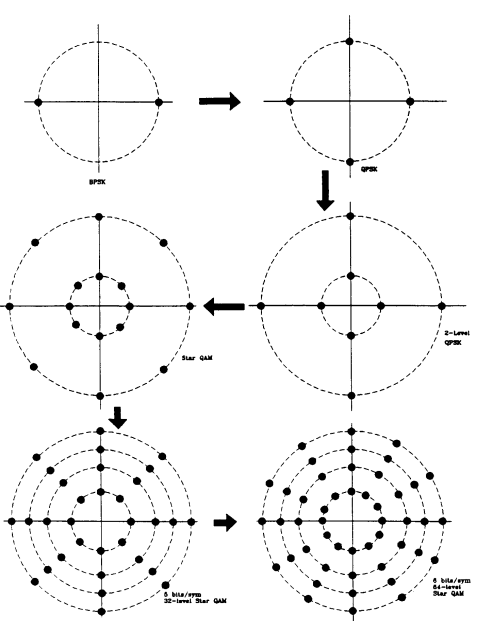
\includegraphics[width=0.45\textwidth]{images/variable_qam.png}
  \caption{Some QAM constellations used in the variable level scheme}
  \label{fig:QAM_examples}
\end{figure}

The capacity of a single DMT line is well established, coming again from Shannon's seminal work\cite{CS48}. His 'ideal' solution, 'Water-filling', simply assigns bit-loads based on the SNR inverse of the line; pouring energy into sub-channels with the best SNR\nomenclature{SNR}{Signal to Noise Ratio}, i.e. most capable of carrying the signal. As the 'best' sub-channels are filled, the adjoining, less capable channels are filled, and so on until no more energy can be added to the channel. 

This is an ideal approach, and presents the maximum theoretical capacity of the line. Practical implementations of this, or any other bit-loading algorithm, must sacrifice 'optimality' for reliability. As such, they must implement what is called a 'Shannon Gap' or 'SNR Gap', a sub-ideal limit on the power loaded on a channel to maintain reliable communications. This subject is revisited in section \ref{sec:XTmodel}, but for the time being, any M-QAM\nomenclature{QAM}{Quadrature Amplitude Modulation} sub-channel constellation, the number of bits that can be encoded within is given in equation ~\ref{eq:MQAMb}\cite{CS48}.

\begin{equation}\label{eq:MQAMb}
b=log_2(M)
\end{equation}

But before going too deeply into the 'problem', first an exploration of the landscape within which the problem lies.

\subsection{DSL System Architecture}
A classical DSL local loop architecture involves a Central Office (CO\nomenclature{CO}{Central Office}), with many Line Termination (LT\nomenclature{LT}{Line Termination, at CO side}) modems,  each connected to a Network Termination (NT\nomenclature{NT}{Network Termination, at CP side}) modem at the Customer Premises (CP\nomenclature{CP}{Customer Premises}). Each LT/NT pair has a separate line between them, and for local loops, these lines are wrapped together in bundles of up to fifty individual lines. This bundle then runs from the CO to the CPs, with intermediate CP lines 'peeling off' the bundle. Additionally, along the length of the bundle, additional lines can 'peel in' to the bundle. Some of the wide variety of possible situations are shown diagrammatically in figures \ref{fig:2-3k5k-nearfar},\ref{fig:4-3k5k-nearfar}.

\begin{figure}[h!]
  \centering
  \subfloat[Possible two line configuration]{\label{fig:2-3k5k-nearfar}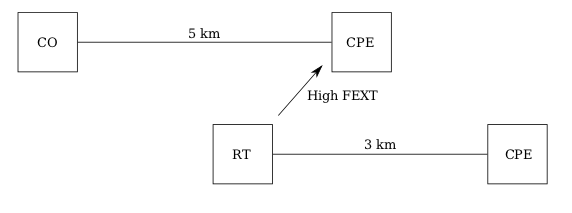
\includegraphics[width=0.45\textwidth]{images/2-3k5k-nearfar.png}}\\
  \subfloat[Possible four line configuration]{\label{fig:4-3k5k-nearfar}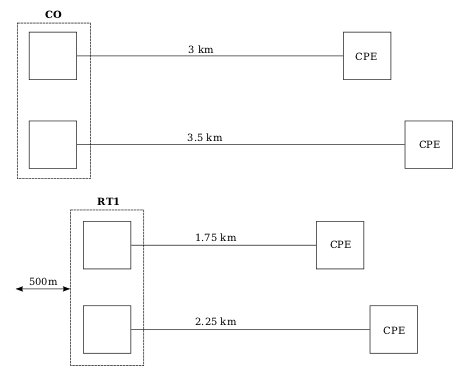
\includegraphics[width=0.45\textwidth]{images/4-3k5k-nearfar.png}}
\end{figure}

These bundles make for a highly noisy RF\nomenclature{RF}{Radio Frequency} environment; with signals from each line interfering with every other line in the bundle through electromagnetic induction of leaked signal power. This phenomenon is termed cross-talk and is the major limiting factor on the achievable data rates of DSL roll-outs, with no current practical solution.

Crosstalk reduces the SNR on DMT sub-channels on a 'victim' line, reducing the amount of bits-per-symbol that can be transmitted on that sub-channel at a pre-defined constant error rate. The level of SNR reduction is often in the 10-20dB range and as such, is the most dominant noise source experienced within the bundle.\cite{RC04}

This phenomenon comes in two major forms; 
\begin{itemize}
  \item Near-End Crosstalk (NEXT\nomenclature{NEXT}{Near End Cross-Talk}): signal leakage from LT-LT or NT-NT
  \item Far-End Crosstalk (FEXT\nomenclature{FEXT}{Far End Cross-Talk}): signal leakage from LT-NT or LT-NT
\end{itemize}

In the vast majority of current DSL roll-outs, NEXT is effectively eliminated through the use of Frequency Division Duplexing(FDD\nomenclature{FDD}{Frequency Division Duplexing}); i.e the upstream data (NT to LT) is sent on a very different frequency than the downstream (LT to NT), and as such does not cause direct interference with a 'neighbouring' termination point.

The amount of cross-talk (XT\nomenclature{XT}{Cross-Talk}) is generally time-constant (excluding severe temperature and humidity changes) and as such can be computationally 'accommodated for' a-priori, but direct vectorisation (we'll find out about that later) and even in-direct cross talk elimination is computationally difficult, if not intractable.

Before one can understand the effects of XT on a DSL system, and especially before one can experiment with different cross talk 'avoidance' algorithms, a realistic dynamic simulation of a functional DSL system must be generated. 

\subsubsection{DSL System Modelling}
Modelling a DSL system, instead of opting for 'real-world' values, allows experimentation and observation of channel behaviours that may not be immediately clear from end-point experimentation \footnote{not to mention that real-world experimentation is time-consuming, expensive, and often incomparable to other results due to a multitude of measurement standards}

Simulation in this case involves the generation of a cross-talk gain (XTG\nomenclature{XTG}{Cross Talk Gain}) matrix for an \(N\)-line network for each of its \(K\) operating channels. This XTG matrix will then be used by the management algorithms to assess the 'cost' or indeed viability of a particular bit-load on a particular line on a particular channel.

As such it is important to understand the electromagnetic transmission characteristics of twisted pair phone lines. This area is largely concerned with the generation of per-line-per-channel transfer functions for interacting sections within a bundle. It is shown in \cite{TS99} that for standard (Category 3) lines, the following RLCG characterisation is stable up to the 30MHz area, at which point this 'simplified' characterisation veers away from real-world performance due to high-frequency envelope shearing. Category 5 lines are stable with this kind of characterisation up to around 150MHz. 

RLCG Characterisation is derived from the per-unit-length two-port model shown in figure ~\ref{fig:rclg}, which can be viewed as a infinitesimally small section of a segment of transmission line. The RCLG parameters represent Resistance, Inductance, Capacitance and Conductance per unit length of line. The direct gain channel models used in this report are based on the long line approximations taken from \cite{AM09}, which in turn were taken from \cite{TS99}.

\begin{figure}[h!]
  \centering
  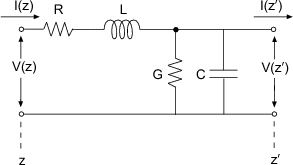
\includegraphics[width=0.25\textwidth]{images/rclg.png}
  \caption{RCLG Characterisation of a two port linear network}
  \label{fig:rclg}
\end{figure}

This assumption is that (for a long DSL line) the input line impedance \(V_1\) matches the characteristic impedance \(V_2\). Given that assumption as well as;
\begin{itemize}
\item \(d\) :line length
\item \(Z\) :Impedance per unit length:\(R \cdot L\)
\item \(Y\) :Admittance per unit length: \(G \cdot C\)
\item \(Z_l\) :load impedance
\item \(Z_s\) :source impedance
\item \(Z_0\) :characteristic impedance:\(\sqrt{\frac{Z}{Y}}\)
\item \(\gamma\) :propagation constant:\(\sqrt{Z \cdot Y}\)
\end{itemize}

The transfer function for a given DSL line is;

\begin{equation}\label{eq:DSLTransferFunc}
H=\frac{Z_0 \cdot \text{sech}(\gamma d)}{Z_s \cdot [\frac{Z_0}{Z_1} +\text{tanh}(\gamma d)]+Z_0 \cdot[1+\frac{Z_0}{Z_1} \cdot \text{tanh}(\gamma d)]}
\end{equation}

To ensure that this modelled transfer function is smooth with respect to frequency \footnote{necessary due to the large margins of error in characterising 'real-world' lines}, the RLCG values are parametrised thus;

\begin{equation}\label{fig:R}
R(f) = \frac{1}{\frac{1}{\sqrt[4]{r^4_{0c}+a_c\cdot f^2}} + \frac{1}{\sqrt[4]{r^4_{0s}+a_s\cdot f^2}}}
\end{equation}

Where \(r_{0x}\) is the DC resistance of copper (c) and steel (s) and \(a_x\) are skin effect related constants

\begin{equation}\label{fig:L}
L(f) = \frac{l_0+l_{\infty}(\frac{f}{f_m})^b}{1+(\frac{f}{f_b})^b}
\end{equation}

Where \(l_x\) are low (0) and high (\(\infty\)) frequency inductance and \(b\) and \(f_m\) define the transition from low to high frequencies.

\begin{equation}\label{fig:C}
C(f)= c_{\infty} + c_0 \cdot f^{-c_e}
\end{equation}

Where \(C_x\) represent contact (\(\infty\)) and other (\(0,e\)) capacitances, chosen from measurements.

\begin{equation}\label{fig:G}
G(f)=g_0\cdot f^{+g_e}
\end{equation}

Where \(G_x\) represent (\(0,e\)) conductances, chosen from measurements.

Within this project, as in \cite{AM09}, AWG 24 line parameters were used, shown in table ~\ref{tab:AWG24Tbl}.

\begin{figure}[h!]
  \centering
  \begin{tabular}{|c|c|c|c|}\hline
    \(r_{0c}=174.56 \Omega\)/km&\(r_{0s}=\infty \Omega\)/km&\(a_c=0.0531\)&\(a_s=0.0\)\\\hline
    \(l_{0}=617.25 \mu H\)/km&\(l_{\infty} = 478.97 \mu H\)/km&\(b=1.1529\)&\(f_m=553.76\)kHz\\\hline
    \(c_{\infty} = 50 \mu F\)/km&\(c_0=0.0\mu F\)/km&\(c_e=0.0\)&\\\hline
    \(g_0 = 234.874 fS\)/km&\(g_e=1.38\)&&\\\hline
  \end{tabular}
  \caption{ETSI Parameters used for AWG24 coaxial lines}
  \label{tab:AWG24Tbl}
\end{figure}


Using these parameters, figure ~\ref{fig:XTG_Example} shows the gain-curve for a variety of lengths of AWG24 cabling produced from equation ~\eqref{eq:DSLTransferFunc}

\begin{figure}[!h]
  \centering
  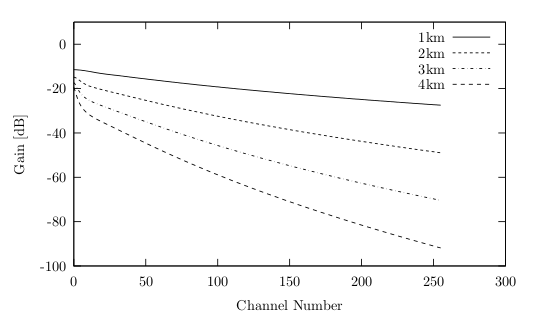
\includegraphics[width=0.45\textwidth]{images/awg24lengths.png}
  \caption{Gain versus channel model for a range of transmission lengths}
  \label{fig:XTG_Example}
\end{figure}

\subsubsection{Crosstalk Modelling}
\label{sec:XTmodel}

The above model allows the generation of 'idealised gains' for a given line, ignoring all external effects, such as the aforementioned cross-talk. To bring cross-talk into the picture, assuming that NEXT is eliminated completely by FDD, we can model FEXT based on the industry standard ETSI 1\% \cite{ETSI03} model (equation ~\eqref{eq:ETSIFEXT})

\begin{equation}\label{eq:ETSIFEXT}
|H_{FEXT}(f)|^2=N^{0.06}K_{FEXT}f^2 |H_{channel}(f,L)|^2
\end{equation}

The "1\%" in this case represents the worst-case-scenario, and in a real deployment would not be encountered 99\% of the time. This is partially driven from systemic pessimism, but partially comes from the fact that this worst-case scenario allows for a modelling function that is smooth with frequency.

In most cases, this 1\% model is over zealous in its estimations of cross-talk coupling, and also ignores spatiality within the bundle \footnote{i.e., lines in the core of the bundle receive much more cross-talk than those on the skin of the bundle}. Using real data from a four sub-bundle, 100x100 DSL binder, the existing model can be modified to more closely match the coupling data of the 'real' bundle.

\begin{equation}\label{eq:ATTFEXT}
|H^{j,k}_{FEXT}(f)|^2=|H^{j,k}_{FEXT}(f)|^2 \times 10^{\frac{X_{dB}}{10}}
\end{equation}

Where the modifier \(X\) is selected based on a Beta probability distribution of sample data, for example, \cite{Alc07}.

As stated, DSL is a cross-talk-limited system, and as such, the effect of cross-talkers also effects some of the fundamental assumptions that must be made about the transmission characteristics of the lines in the bundle.

From \cite{SJ08}, the approximate Shannon Gap for a DSL system based on M-QAM is derived thus. From the Central Limit Theorem, as the number of cross-talkers increases, the effects of those cross-talkers approximates to a Gaussian Distribution\cite{KK93}. Therefore, a DSL channel can be approximated as an Additive White Gaussian Noise (AWGN) channel, which is described \cite{CS48}:

\begin{equation}\label{eq:AWGN}
C(k)=log_2(1+SNR(k))
\end{equation}

This represents the maximum possible capacity (in bits) on a given channel (\(C(k)\)), ignoring practical considerations such as coding complexity and processing delays. From \cite{CS48} and \cite{JMC91}, the probability of a symbol error for an uncoded M-QAM constellation \footnote{with an associated number of nearest neighbours, \(N_e\)} on a given sub-channel is shown in equation ~\eqref{eq:PeMQAM}

\begin{equation}\label{eq:PeMQAM}
P_e\approx N_eQ\left(\sqrt{\frac{3}{M-1}SNR}\right)
\end{equation}

Where \(Q(x)\) is the probability of unitary Gaussian variable will will exceed \(x\), given in equation ~\eqref{eq:QxQAM}. In general, DSL systems aim for this probability of symbol error (\(P_e\)) to be around \(1e^{-7}\).

\begin{equation}\label{eq:QxQAM}
Q(x)=\int_x^{\infty}\frac{1}{\sqrt{2\pi}}e^{-u^2/2} du
\end{equation}

\eqref{eq:QxQAM} is generally rewritten in terms of the standard error function \(erf(x)\), shown in equations ~\eqref{eq:QxQAMerf} and ~\eqref{eq:QxQAMerf2}.

\begin{equation}\label{eq:QxQAMerf}
Q(x)=\frac{1}{2}\left(1-erf(\frac{x}{\sqrt{2}})\right)
\end{equation}

\begin{equation}\label{eq:QxQAMerf2}
Q^{-1}(x)=\sqrt{2} erf^{-1}(1-2x)
\end{equation}

Rearranging ~\eqref{eq:PeMQAM} for \(M\) gives ~\eqref{eq:QAM4M}

\begin{equation}\label{eq:QAM4M}
M=1+\frac{SNR}{\frac{1}{3}(Q^{-1}(\frac{P_e}{N_e})^2)}
\end{equation}

Revisiting ~\eqref{eq:MQAMb}, ~\eqref{eq:MQAMbmax} can be obtained, expressing the number of bits that can be encoded on a sub-channel.

\begin{equation}\label{eq:MQAMbmax}
b=log_2\left(1+\frac{SNR}{\frac{1}{3}(Q^{-1}(\frac{P_e}{N_e})^2)}\right)
\end{equation}

Contrasting ~\eqref{eq:MQAMbmax} with ~\eqref{eq:AWGN}, the uncoded channel gap is defined in equation ~\eqref{eq:GAMMAuncoded}.

\begin{equation}\label{eq:GAMMAuncoded}
\Gamma_{uncoded}=\frac{1}{3}\left(Q^{-1}(\frac{P_e}{N_e}\right)^2
\end{equation}

This allows simplification of equation ~\eqref{eq:MQAMbmax} with respect to ~\eqref{eq:GAMMAuncoded} into ~\eqref{eq:GAMMAb}

\begin{equation}\label{eq:GAMMAb}
b=log_2\left(1+\frac{SNR}{\Gamma_{uncoded}}\right)
\end{equation}

This characterisation of the Shannon Gap is not quite complete, and represents the best-case scenario within a DSL system, while ignoring potential coding gains from Forward Error Correction such as the Trellis\cite{GU82} or Reed-Solomon\cite{Ree59} coding schemes.

As such, two additional modifiers are added to the \(\Gamma\) calculation; a performance margin \(\gamma_m\) which allows for SNR 'headroom' to maintain error rates during temporarily bad noise conditions, and a coding gain \(\gamma_{eg}\) which incorporates any error correction modulation in place. This gives a final \(\Gamma\) sum shown in equation ~\eqref{eq:GAMMAsum}

\begin{equation}\label{eq:GAMMAsum}
\Gamma=\Gamma_{uncoded}+\gamma_m+\gamma_{eg}
\end{equation}

In \cite{AM09} it is demonstrated that cross-talk coupling can be assumed not to have any practically relevant effect on sub-channels other than the sub-channel from which that cross-talk originates, such as when DMT blocks are transmitted and received synchronously or when cyclic prefixing and pulse shaping ("Zipper" DMT\cite{FSJ99}) is used.

From \cite{CA06}, equation ~\eqref{DSLSystemModel} shows the maximally optimal bit-loading on line \(n\) of \(N\) users, and tone \(k\) of \(K\) total sub-channels, including the above derivation for FEXT coupling.

\begin{equation}\label{DSLSystemModel}
b_n(k)=log_2\left(1+\frac{p_n(k) |h_{nn}(k)|^2}{\Gamma \left( \sigma_n^2(k)+\sum_{j\neq n}^N p_j(k)|h_{jn}(k)|^2 \right)} \right)
\end{equation}

In equation ~\eqref{DSLSystemModel}, the following definitions are provided for clarity;

\begin{itemize}
  \item \(h_{ij}(k)\)\nomenclature{\(h_{ij}(k)\)}{XTG from user \(i\) to user \(j\) on channel \(k\) }:The cross-talk gain from user \(i\) to user \(j\) on channel \(k\)
  \item \(p_n(k)\)\nomenclature{\(p_n(k)\)}{Power provisioned on channel \(k\) for user \(n\)} :The power provisioned on channel \(k\) for user \(n\)
  \item \(\sigma^2_n(k)\)\nomenclature{\(\sigma^2_n(k)\)}{Background noise power experiences by user \(n\) on channel \(k\)} :The background noise power experienced by user \(n\) on channel \(k\)
  \item \(\Gamma\)\nomenclature{ \(\Gamma\)}{The Shannon Gap derived from equation \eqref{eq:GAMMAsum}}:The Shannon Gap derived from ~\eqref{eq:GAMMAsum}
\end{itemize}

By letting \(f(b_n(k))=\Gamma(2^{b_n(k)}-1)\), ~\eqref{DSLSystemModel} can be rearranged to ~\eqref{eq:DSLSystemModelAlt}

\begin{equation}\label{eq:DSLSystemModelAlt}
p_n(k)-f(b_n(k))\sum_{j\neq n}^N p_j(k) \frac{|h_{jn}(k)|^2}{|h_{nn}(k)|^2}=f(b_n(k))\frac{\sigma_n^2(k)}{|h_{nn}(k)|^2}
\end{equation}

It is clear that equation ~\eqref{eq:DSLSystemModelAlt} can be characterised as an N-dimensional linear system of equations, of the form 

\begin{equation}\label{eq:SysModMat}
A(k)P(k)=B(k)
\end{equation}

Where

\begin{equation}\label{eq:SysModA}
A(k)_{ij}=\begin{cases} 1, & \mbox{for } i = j \\\frac{-f(b_i(k))|h_{ji}|^2}{|h_{ii}|^2}, & \mbox{for } i \neq j \end{cases}
\end{equation}

\begin{equation}\label{eq:SysModP}
P(k)=[p_1(k) \dots p_i(k) \dots p_N(k)]^T
\end{equation}

\begin{equation}\label{eq:SysModB}
B(k)=\left[\frac{f(b_1(k)) \sigma^2_1}{|h_{11}|^2} \dots \frac{f(b_i(k)) \sigma^2_i}{|h_{ii}|^2} \dots \frac{f(b_N(k))\sigma^2_N}{|h_{NN}|^2}\right]^T
\end{equation}

As such, the vector \(B(k)\), as a function of \(b(k\), describes the amount of bits loaded onto each user's line on tone \(k\), and \(P(k)\) prescribes the power required on each line to support the vector \(B(k)\) of bits loaded onto those lines on channel \(k\). It is the solution and optimisation of this system of equations that is the fundamental limiting factor, and drive for, DSM systems. 

The reasoning for this is primarily visible looking at the concept of rate-regions, i.e an \(N\)-dimensional surface of possible maximum line bit-loads for each user \(n\). Figure ~\ref{fig:RateRegionExample} shows the relationship between two given users, \(R_1\) and \(R_2)\) within a given bundle. It is evident that one \emph{could} achieve an very high data-rate on one line, but at great expense to the other. Mathematically, the search for optimal bit-loading is summed up in ~\eqref{fig:RateRegionEqu}.

\begin{figure}[h!]
  \centering
  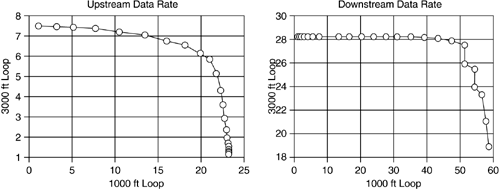
\includegraphics[width=0.75\textwidth]{images/rateregion.png}
  \caption{Example of a ADSL rate Region for two users from \cite{TS03}}
  \label{fig:RateRegionExample}
\end{figure}

\begin{equation}\label{fig:RateRegionEqu}
\max\limits_{\{p_n\in P_n\}_n} \sum_n w_n R_n
\end{equation}

Using an optimal rate-region, of the style demonstrated in equation ~\ref{fig:RateRegionEqu} can be generated algorithmically from the above equations. But often these algorithms can be computationally intractable, and less computationally expensive (but sub-optimal) algorithms are used instead, producing reduced rate regions which do not take full advantage of the available spectrum given the same cross-talk and bundle noise characteristics.

In essence, this Spectrum Management Problem, as stated in equation ~\eqref{fig:RateRegionEqu}, can be expanded based on line-weighting; where some lines get 'preferential treatment', either because they are paying more, or as part of a lead-and-lag rate-compensation system\footnote{Lag and Lead, terms originally from the field of economics but 'adopted' by the field of control theory, implies a kind of 'lending' system, where by a given variable (in this case the bit-rate/weight on a particular line) can be allowed to 'run rampant' if the system has spare capacity, but that added usage is accounted and is 'paid back' to the system when needed, and often that particular variable will be more 'borrowed from' until its lag/lead accounts are even again}. Thus, the Spectrum Management Problem can be generalised to \(N\) users as a maximisation of a weighted sum of data rates within a bundle, as shown in equation ~\eqref{fig:WeightedDSLSystemModel}.

\begin{equation}\label{fig:WeightedDSLSystemModel}
\begin{array}{rc}
\sum\limits_{n=1}^N w_n \sum\limits_{k=1}^K & log_2 \left(1+\frac{p_n(k_|h_{nn}(k)|^2}{\Gamma\left(\sigma_n^2(k)+\sum\limits_{m\neq n}^N p_m(k)|h_{jm}(k)|^2\right)}\right)\\
 &s.t.\sum_{k=1}^Kp_n(k) \leq P_{max,n} \forall n
\end{array}
\end{equation}

The optimisation of this problem in a dynamic near-realtime time-frame is the major focus of DSM research, which is summarised next.


\subsection{Dynamic Spectrum Management Introduction}
A general solution to this rate-region problem has been the use of Static Spectrum Management (SSM), where each line has a pre-defined power spectral density (PSD\nomenclature{PSD}{Power Spectral Density}) profile under which it operates. This is sometimes called Spectral Masking. Unfortunately this masking is done once (or a few times, if lines are added to / removed from the bundle), and additionally assumes that each line will be fully utilised at all times. This a major abstraction from reality, and has driven the development of spectrum management systems that can dynamically re-allocate PSD's based on near-real-time usage. From \cite{STC07}:

\begin{quotation}
Suppose that 25 copper lines exist in a cable bundle. Depending on the time (day versus night, weekday versus weekend) and the location (commercial versus residential area), the demand for DSL services varies. For example, the data traffic load at an office is heavy during the daytime and may be close to zero at night. Furthermore, depending on the specific loop topologies, the interference caused by one line to another varies. Some pairs might be physically close in the binder over a very short distance; hence, the interference between these pairs might be very small. On the other hand, other pairs might be proximate along most of the loop length, which leads to a very strong interference between those two pairs
\ldots
Revisiting the example where 25 copper lines exist in a telephone bundle, suppose that in the middle of the night at school, one Ph.D. student is trying to download a large paper from a website using DSL. If static spectrum management is used, the speed is as slow at night as during the day, when many other students are also using their DSLs. However, if the DSL network uses [Dynamic Spectrum Management], the speed at night can be much faster than during the daytime because the bit-rate on the line in use can be optimised to take advantage of the low-noise conditions.
\end{quotation}

It is clear that with the addition of some usage-based intelligence, the bundle could be much more effectively used. Dynamic Spectrum Management systems allow for power and rate allocations for each line to be dynamically controlled, but are classified into four general levels, based on the amount of coordination between lines, ranging from completely autonomous operation\footnote{Strictly speaking not DSM but included for completeness} to centralised signal vectoring and control, as summarised in Figure \ref{tab:DSMLevelTable}, adapted from \cite{JC06} and \cite{AM09}.

\begin{figure}[h!]
  \begin{minipage}{\textwidth}
\begin{tabularx}{\textwidth}{c|X|p{3cm}|}
  DSM Level&Description&Examples\\\hline
  0&No DSM, Completely Autonomous per-modem Spectrum Management&NA \\
  1&Single line spectrum balancing with politeness and signal impulse control&IWF\footnote{Iterative Water Filling},ASB\footnote{Autonomous Spectrum Balancing}\\
  2&Multiple line spectrum balancing with spectra controls&OSB\footnote{Optimal Spectrum Balancing}, ISB\footnote{Iterative Spectrum Balancing},SCALE\footnote{Successive Convex Approximation for Low ComplExity\cite{Pap06}}\\
  3&Multiple line signal coordination (vectoring)&Vectored-DMT\cite{GG00}, SVD\footnote{Single Vector Decomposition\cite{GTaWH00}}\\
\end{tabularx}
\end{minipage}
\caption{Summary of DSM Algorithm Level Characteristics with Examples}
\label{tab:DSMLevelTable}
\end{figure}


This coordination (where applicable) is controlled centrally from a Spectrum Maintenance Centre (SMC\nomenclature{SMC}{Spectrum Maintenance Centre}), which receives data from Customer Premises Equipment (CPE\nomenclature{CPE}{Customer Premises Equipment}) via an Auto-Configuration Server (ACS\nomenclature{ACS}{Auto-Configuration Server}), and/or from DSLAMs\nomenclature{DSLAM}{DSL Access Multiplexer} and LT-side equipment via an Element Management System (EMS\nomenclature{EMS}{Element Management System}). The SMC then collates the received information, and distributes profile settings for the DSLs.

\subsection{DSM Level 0/1}
For clarity, levels 0 and 1 are generally grouped, as the only major difference is that while in level 0\footnote{currently the most common method of 'Spectrum Balancing'}, equipment is completely autonomous in terms of its own spectrum management; level 1 systems receive power and rate limitations from the SMC, within which they must operate. Level 0 is currently the most commen method of DSM utilised currently, but some ISPs are moving to level 1 systems, such as Virgin.

Thinking back to the initial discussion of DMT spectrum balancing, the most common technique for autonomous spectrum assignments is based on Water-filling \cite{CS48}, and refined for DSL in \cite{WYaJC00} \cite{WY01}

For the single user case, refer to figure ~\ref{fig:WaterFillingSingleExample}, but in the multi-user case, water-filling attempts must be iteratively refined (Hence, Iterative Water-Filling, or IWF\nomenclature{IWF}{Iterative Water-Filling}); so as to allow the 'other' lines to see each lines new noise profile, see figure ~\ref{fig:WaterFillingMultiExample} for a graphical example of this. This helps to reduce the effects of the so-called "Near Far Problem", whereby the received signal from cross-talker which is closer to the receiver, is stronger than its direct line transmitter signal.

\begin{figure}[h!]
  \centering
  \subfloat[Single User]{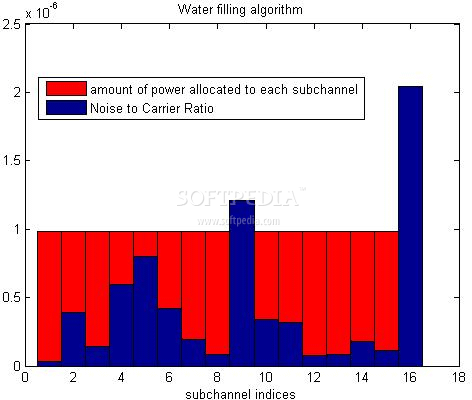
\includegraphics[width=0.5\textwidth]{images/wf.png}\label{fig:WaterFillingSingleExample}}
  \subfloat[Iterative Multiple User]{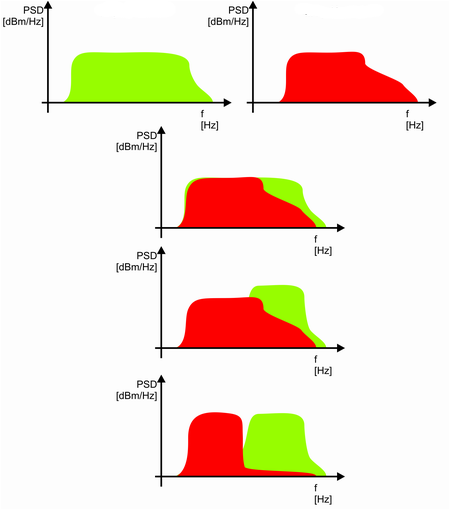
\includegraphics[width=0.4\textwidth]{images/iwf.png}\label{fig:WaterFillingMultiExample}}
  \caption{Example of Water Filling}
\end{figure}

The water-filling algorithm produces the optimal solution\footnote{It is proven in \cite{STC03} that for frequencies less than 2MHz, there exists only one Nash Equilibrium point within a distributed DSL network, and although it is possible, no example of multiple optimal rate-region points has been discovered to date \cite{STC07}}, maximising channel capacity for a single user with a continuous bit-assignment \footnote{I.e non-integer bit-assignments are permitted}. In practise this is incorrect, as integer bits must be assigned to each channel for transmission. When this integer condition is applied, it is known as "Discrete Water-filling". Discrete water-filling has two variations; one which focuses on maximising bit-rate with respect to a stated power budget, known as Rate-Adaptive (RA\nomenclature{RA}{Rate Adaptive water filling}); and another which focuses on minimising the power requirements with respect to a stated bit-rate, known as Fixed-Margin (FM\nomenclature{FM}{Fixed-Margin water filling}). These two conditions are mathematically phrased in ~\eqref{RADefine} ~\eqref{FMDefine}\cite{TS99}.

\begin{equation}
  \begin{array}{rcl}
  max R&=&\sum_{k=1}^Kb(k)\\
  s.t.&&\sum\limits_{k=1}^Kp(k)\leq P_{budget}
  \end{array}
\label{FMDefine}
\end{equation}

\begin{equation}
  \begin{array}{rcl}
  min &&\sum\limits_{k=1}^Kp(k)\\
  s.t.&&\sum\limits_{k=1}^Kb(k)\geq B_{budget}
  \end{array}
\label{RADefine}
\end{equation}

The resolution of both of these forms of water-filling is surprisingly simple in theory; find the tone with the lowest bit-addition energy \footnote{generally termed \(\Delta p(k)\)\nomenclature{\(\Delta p(k)\)}{Single-bit addition power}}, and add a bit to it. This continues until either the power or rate budget is reached, depending on the mode applied. This basic algorithm is the Levin-Campello (LC\nomenclature{LC}{Levin-Campello Algorithm}) Algorithm\cite{H.L01}.

\subsubsection{Iterative Water Filling}
One of the first forms of DSM, IWF is computationally simple, de-centralised, and relatively easy to implement.
The rational of IWF is to limit iteratively perform LC bit-loading and to adapt the power constraints so as to limit the power used in the bundle while maintaining total bundle capacity, thereby lowering the power of cross-talking signals and actually increasing the net bundle data rate greatly when compared to SSM\nomenclature{SSM}{Static Spectrum Management}, but is far from optimal, and is not guaranteed to converge, or settle, on on any result. The general algorithm for IWF is shown in figure \ref{fig:IWFAlgorithm}

\begin{figure}[h!]
\begin{algorithmic}
\REPEAT
\FOR{n=1...N}
\STATE Execute LC Algorithm with power budget \(P_n\) on line \(n\)
\IF{\(R_n>R_n^{target}\)}
\STATE \(P_n=P_n-\gamma\)
\ELSE
\STATE \(P_n=P_n+\gamma\)
\ENDIF
\ENDFOR
\UNTIL{convergence}
\end{algorithmic}
\caption{IWF Algorithm}
\label{fig:IWFAlgorithm}
\end{figure}

\subsection{DSM Level 2}
\subsubsection{Optimal Spectrum Balancing}
From \cite{RC04}, OSB optimally solves the Spectrum Management Problem for multiple users, but is highly computationally intensive and generally cannot be practically computed for more than four lines \cite{AM09}. The avenue taken by OSB in solving the Spectrum Management Problem is a mathematically complex one. The solution is centred around the use of a Lagrangian dual decomposition of the initially states Spectrum Management Problem ~\eqref{fig:WeightedDSLSystemModel}. To explain what this process entails, one must look closer at the problem; from \cite{RC04}

\begin{quotation}
  The fundamental problem is that the total power constraints on the modems couple the optimisation across frequency. As such optimisation must be done jointly across all tones, which leads to an exponential complexity in \(K\). We overcome this problem through the use of the dual decomposition method. This technique allows us to replace the constrained optimisation problem with an unconstrained maximization of a Lagrangian\footnote{A Lagrangian of a dynamical system is a function that summarises the dynamics of the system, and in the field of optimisation, allows for the joint-optimisation of a dually (in this case) constrained problem through the use of an additional Lagrange multiplier to generate the new Lagrangian decomposition \(L\) that implicitly encompasses both (all) constraint functions} The Lagrangian incorporated the constraints implicitly into the cost function, removing the need for the constraints to be explicitly enforces. As a result, the optimisation can be decoupled across frequency, and an optimal solution can be found in a per-tone fashion. This leads to a linear rather than exponential complexity in \(K\) and a computationally tractable problem.
\end{quotation}
 
In practical terms, that means that the Spectrum Management Problem can be 'simplified' to include the pan-channel power constraints, meaning that instead of generating many solutions to the general (first line of ~\eqref{fig:WeightedDSLSystemModel}) problem, and then subsequently discarding those as they do not satisfy the bundle power constraints, global power is a focal consideration. The Lagrangian decomposition of ~\eqref{fig:WeightedDSLSystemModel}, encompassing the power constraints, is shown in ~\eqref{fig:LagrangianModel}

\begin{equation}
L=\sum\limits_{n=1}^N w_n \sum\limits_{k=1}^K log_2 \left(1+\frac{p_n(k_|h_{nn}(k)|^2}{\Gamma\left(\sigma_n^2(k)+\sum\limits_{m\neq n}^N p_m(k)|h_{jm}(k)|^2\right)}\right)-\lambda_n\left(\sum\limits_{k=1}^K p_n(k)\right)
\label{fig:LagrangianModel}
\end{equation}

Is was shown by Yu and Lui\cite{WYaRL06} that this decomposition is an exact match to the originally stated problem for large numbers of channels.

It is also stated in \cite{AM09} that ~\eqref{fig:LagrangianModel} can be tonally decoupled, and a (unfortunately non-convex) Lagrangian expression for each channel generated, as in ~\eqref{fig:LagrangianDecoupled}, and by optimising for a maximal per-tone Lagrangian, and searching \(\lambda\) space\footnote{How the \(\lambda\) space is searched is a matter of much debate, which will be met later}, the original problem can be solved.

\begin{equation}
  L(k)\nomenclature{\(L_k\)}{The Lagrangian sum of a bitloaded channel}=\sum\limits_{n=1}^Nw_nb_n(k)-\sum\limits_{n=1}^N\lambda_np_n(k)
\label{fig:LagrangianDecoupled}
\end{equation}

Since ~\eqref{fig:LagrangianDecoupled} is non-convex, an exhaustive search across \(b_n\) space is required\footnote{For the interested reader, this is a computationally explosive procedure; consider the vector \(B(k)\), with each vector index as the bit load on a particular line on channel \(k\), and a maximum bits per tone of 15 (from the DSL standard). For two lines, this represents only 225 possibilities, but for four, its 50625; for 8 its over 2.5 billion, and for a standard 50 line bundle, its a 59 digit number.To put that in perspective, the number of stars in the observable universe is only a 24 digit number. For a given max bits per tone \(b_{max}\), the number of bit combinations for \(N\) lines is \(b_{max}^{N}-1\)}
Even with the Lagrangian decomposition, the computationally explosive nature of this exhaustive bit-field search renders OSB computationally intractable for more than four or five lines. Some run-times from \cite{AM09} are shown in figure ~\ref{tab:TractibilityTable}

The generalised algorithm for OSB is shown in figure \ref{fig:OSBAlgorithm}

\begin{figure}[!h]
\begin{algorithmic}
\REPEAT
\REPEAT
\FOR{\(k=1\dots K\)}
\STATE \(\arg\max_{b_(k)}L(k)=\sum_{n=1}^Nw_nb_n(k)-\sum_{n=1}^N\lambda_np_n(k)\)
\STATE Solve by N-d exhaustive search
\ENDFOR
\STATE \(\lambda_n=\lambda_n+\epsilon(\sum_{k=1}^Kp_n(k)-P_n^{max})\)
\UNTIL{\(\lambda\) convergence}
\STATE \(w_n=w_n+\epsilon(\sum_{k=1}^Kb_n(k)-R_n^{target})\)
\UNTIL{\(w\) convergence}
\end{algorithmic}
\caption{OSB Algorithm}
\label{fig:OSBAlgorithm}
\end{figure}

OSB can be augmented using a Branch and Bound searching structure into Branch and Bound OSB (BBOSB). BBOSB is covered in detail in \cite{PT06}, but suffice to say, even with the improved searching structure, BBOSB is still exponential in \(N\), but with a lower complexity coefficient; where OSB is only tractable for 4-5 lines, BBOSB is tractable up to approximately 10 lines \cite{AM09}.

\subsubsection{Iterative Spectrum Balancing}
ISB is based on the same Lagrangian decomposition as OSB, but instead of an exhaustive search across the bit-space within the Lagrangian, each line in turn is optimised, i.e a linear search instead of OSB's \(N\)-vector-search. It was presented\cite{Cen05} by Cendrillon and Moonen in 2005 and thoroughly investigated by Yu and Lui\cite{WYaRL06} in 2006, and is near-optimal, but is not guaranteed to converge on a global maximum.\cite{Cen05}.

The improvement in computational complexity is great; OSB has a \(N\) complexity of \(O(b_{\text{max}}^N)\), whereas ISB attains a complexity of \(O(N^2)\), meaning that for slightly more practical bundle sizes, ISB is computationally tractable. The ISB algorithm is shown in figure ~\ref{fig:ISBAlgorithm}

\begin{figure}[h!]
\begin{algorithmic}
\REPEAT
\FOR{\(k=1\dots K\)}
\REPEAT
\FOR{\(n=1\dots N\)}
\STATE Fix \(b_m(k)\forall m \neq n\)
\STATE \(\arg\max_{b_(k)}L(k)=\sum_{n=1}^Nw_nb_n(k)-\sum_{n=1}^N\lambda_np_n(k)\)
\STATE \(\lambda_n=\lambda_n+\epsilon(\sum_{k=1}^Kp_n(k)-P_n^{max})\)
\STATE Solve by 1-d exhaustive search
\ENDFOR
\UNTIL{\(\lambda\) convergence}
\ENDFOR
\STATE \(w_n=w_n+\epsilon(\sum_{k=1}^Kb_n(k)-R_n^{target})\)
\UNTIL{\(w\) convergence}
\end{algorithmic}
\caption{ISB Algorithm}
\label{fig:ISBAlgorithm}
\end{figure}

\subsubsection{Multi-User Greedy Spectrum Balancing}
It has been shown that while the LC algorithm is optimal in the case of a single line, the straightforward multi-user expansion of this (IWF) is decidedly sub-optimal. Cioffi, Sonalkar, and Lee, in \cite{JL05} presented a heuristic extension to the Levin-Campello Algorithm, termed Multi-User Greedy Spectrum Balancing. 
The heuristic applied was, instead of in IWF where each line is individually optimised, the bundle is viewed as a whole, and bits are iteratively assigned to both the line and channel with the minimum cost of addition.
This cost of bit-incrementing, which for IWF was simply \(\Delta p_m(k)\) where \(m\) was the line being balanced, and \(k\) was the channel on the line with the lowest additional power requirement; additionally includes the sum of \(\Delta p_n(k)\) on all other lines required to accommodate the additional cross-talk generated on the incremented line ~\eqref{eq:GreedyCost}.

\begin{equation}
C(m,k)=\sum\limits_{n=1}^N\left(\underset{p_n(k)}{b(k)+1} - \underset{p_n(k)}{b(k)}\right)
\label{eq:GreedyCost}
\end{equation}

\subsubsection{Multi-User Incremental Power Balancing}
In \cite{AM09}, McKinley details the development of MIPB as coming from a critical analysis of Multi-User Greedy Spectrum Balancing. One of the major deficiencies of Greedy is the (significant) possibility of the algorithm getting stuck in local minima, or getting 'deadlocked', whereby bits cannot be added to any lines due to any other line in the bundle attempting to violate  its power constraint to accommodate the additional cross talk incurred, (see ~\ref{eq:GreedyCost}). To remedy this, an adaptive power penalty function is used to stop 'clean' lines being continuously loaded up to their power budget, and then 'locking' all other lines, and to instead force all the lines to be more or less equalised as the algorithm progresses. The algorithm for MIPB is shown in figure \ref{fig:MIPBAlgorithm}. The final bundle efficiency of MIPB, while non-optimal, is very close, but the real improvement is in runtime performance; 10 lines with rate targeting applied in under five minutes.

\begin{figure}[h!]
\begin{algorithmic}
\REPEAT
\STATE \(\text{argmin}_{n,k} C\)
\STATE \(b_n{k}=b_n{k}+1\)
\FOR{\(n=1\dots N\)}
  \STATE \(\delta p_{n,k}=\left(\underset{p_n(k)}{b(k)+1} - \underset{p_n(k)}{b(k)}\right)\)
\ENDFOR
\FOR{\(n=1\dots N\)}
  \FOR{\(k=1\dots K\)}
    \STATE \(C_{n,k}=\sum\limits_{n=1}^N \text{wp}(n)\times\delta p_{n,k}\)
    \STATE Where wp\(n\) is a power penalty function
  \ENDFOR
\ENDFOR
\UNTIL All tones full
\end{algorithmic}
\caption{MIPB/Greedy algorithm}
\label{fig:MIPBAlgorithm}
\end{figure}

\begin{figure}[h!]
  \begin{tabularx}{1.1\textwidth}{|X|c|c|c|c|c|c|c|c|}\hline
  &&\multicolumn{7}{|c|}{N-User Runtimes (s/sec,m/min,h/hrs)}\\\hline
  Algorithm&Complexity&2&3&4&5&6&7&8\\\hline
  OSB&\(O(K b_{\text{max}}^N N^3)\)&35.65s&3.24h&*&*&*&*&*\\\hline
  OSB (Cached)&\(K b_{\text{max}}^N N^3)\)&14.6s&2.12h&*&*&*&*&*\\\hline
  ISB&\(O(K N^2 N^3)\)&32.31s&16.22m&3.93hrs&12.06h&8.69h&28.46h&*\\\hline
  ISB (Cached)&\(O(K N^2 N^3)\)&2.73s&53.57s&9.35m&30.04m&26.74m&1.42h&*\\\hline
  BBOSB&\(O(K b_{\text{max}}^N N^3)\)&7.12s&15.73m&13.04h&*&*&*&*\\\hline
  BBOSB (Cached)&\(O(K b_{\text{max}}^N N^3)\)&2.88s&4.2m&3.12h&*&*&*&*\\\hline
  MIPB Bisection&\(O(B_{\text{total}} N^2 N^3)\)&0.26s&9.99s&35.6s&3.71m&12.88m&6.36m&51.72m\\\hline
  MIPB (Cached)&\(O(B_{\text{total}} N^2 N^3)\)&0.19s&3.89s&10.96s&49.97s&*&*&*\\\hline
\end{tabularx}
\caption{Adapted from McKinley '09, 'Caching' implies the use of PSD key-value caching, and * signified unmeasured/invalid execution times}
\label{tab:TractibilityTable}
\end{figure}


\subsection{DSM Level 3}
Level 3 techniques rely on the concept of signal vectoring, coordinated at a DSLAM, such that all lines are terminated on common equipment. Complete signal vectoring eliminates cross-talk through the generation of a cancellation matrix consisting of block-permuted, diagonal Inverse Discrete Fourier Transform matrices, acting as a Generalised Decision Feedback Equaliser, which, as demonstrated in \cite{Cio97}, can eliminate cross-talk, as well ISI in the case of impulse envelope skewing over long lines.

Vectored-DMT (VDMT\nomenclature{VDMT}{Vectored DMT}) can produce optimal bundle efficiencies, but the conditions on VDMT's operation\footnote{Co-location of at least one side of the bundle, computationally expensive pre-computation, inflexibility of applications, requirement for expensive real-time DSP hardware at both bundle terminations} make it inapplicable for commercial use.

Fortunately, DSL Level 3 is not the subject of this project.

\section{Parallel Computing}\label{sec:ParallelComputing}
Today, most (hopefully all) engineering and computer science students are educated in programming, in one form or another. The current languages of choice;C,C++, Java, and Python, all (classically) conform to what is known as procedural, or imperative, programming, where by instructions are written to be serially fed into a processor, and data flow is dictated by run-time conditional redirection. Ever since the computing innovations of Turning in the 1940's\cite{Tur36} and the later codification of the Von Neumann Architecture (VNA) after his work on EDVAC \footnote{Electronic Discrete Variable Automatic Computer, predominantly used for Ordnance Trajectory calculations and other military applications}\cite{VN45}, the concept of a serially operated computers dominated the field of computer science for decades.

Parallel computing, on the other hand, which simultaneously uses many processing units to solve a problem by breaking the problem (or data) set up and distributing this split workload to different processing units\footnote{Whether instruction pipe-lining should be included in this is a point of debate, which will be dealt with later in this chapter}, has been a niche interest. Parallel computing was for a long time the reserve of a few highly specialised machines created over the years, generally in the fields of medicine, energy or warfare.\footnote{For example, the Cray-1 was built for fusion plasma dynamics research, the Cytocomputer pipelined processor was built for biomedical image processing in 1980 \cite{RML80}, and the Staran Content-Addressable Parallel computer, built in 1972, was used for Cartographic data processing for military intelligence\cite{KH84}}

The reason for this 'edging out' of parallel computation was simple; Moore's Law\cite{Moo65}. In 1965, Moore, then at the newly formed Fairchild Semiconductor, posited that computational density doubles more-or-less every 18 months. This pattern has held for about four decades. This continuous, explosive, growth drove programmers with computationally intense problems simply to wait 18 months for their applications to run twice as fast on newer hardware, instead of using problem decomposition to solve the current problem in a more distributed way. This period of exponential processing growth in respect to hardware has, in recent years, come up against major blocks; quantum physics\footnote{Quantum Tunnelling leads to non-deterministic behaviour at around the 16 nanometre mark\cite{Zhi03}}, the infamous 'power wall'\footnote{If processor speeds were growing today at the same rate as in the mid-90's, CPU's would require a power density equivalent to that of a Saturn V booster stage nozzle\cite{Rab07}}, and a general consumer and industrial drive towards low power devices (including 'supercomputers').

Since the early 2000's, the semiconductor industry has settled on two main paths to stave-off the demise of Moore's Law (in its current form\footnote{Moore himself has said 'his' law is the exception to Murphy's Law, in that no-matter what doomsday predictions are made regarding it, The Law seems to perpetuate itself in new forms}); multi-core and many-core. 

Multi-core processing involves the use of a relatively small number of monolithic processing units, very akin to traditional single CPU's, placed on a single die, maintaining the execution speed of existing sequential programs while allowing for direct execution concurrency at lower clock-rates (and hence power) than a similarly scaled single core processor. The latest 'state of the art' in this field is the Intel i7 Sandy Bridge 32nm architecture, with 8 processing cores\cite{Var11}, each of which is a hyper-threaded\footnote{Read:two hardware threads per core} x86 instruction set processor, giving, in theory, 16 hardware threads of parallelism. The trend in these types of devices has actually almost matched Moore's Law in its simplest form; the number of cores in multi-core chipsets has been roughly doubling every two years.

Many-core computing, on the other hand, involves the use of a relatively large number of 'dumb' cores. While many many-core architectures exist\footnote{IBM's BlueGene/Q architecture, Intel's Larabee Microarchitecture, AMD's FireStream, NVIDIA's Tesla, and Tilera's iMesh to name a few} the area in which parallel computing research and applications has been recently most focused is the development and adaptation of consumer graphics hardware to application acceleration and scientific computing, termed General Purpose computing on GPU's (GPGPU).

\begin{figure}[h!]
  \centering
  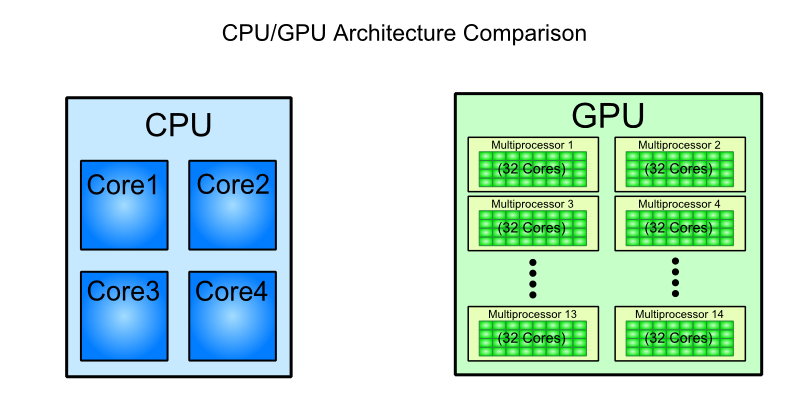
\includegraphics[width=0.75\textwidth,keepaspectratio=true]{images/cpu_vs_gpu.png}
  \caption{Multicore CPU's and Manycore GPU's have fundamentally different design philosophies}
  \label{fig:CPUvsGPU}
\end{figure}

The real difference between multi-core and many-core computing can be seen in Figure ~\ref{fig:CPUvsGPU}, whereby a multi-core CPU, such as the Intel Core i5, has a number of large distinct Processing Units (PUs\nomenclature{PU}{Processing Unit}), whereas an NVidia GPU\footnote{Used as an example of Many-core computing; the general principals apply across many-core devices} consists of an array of many smaller Streaming Multiprocessors (SM) that themselves contain an array of Streaming Processors (SP\nomenclature{SP}{Streaming Processor})\footnote{These principals will be covered in more detail in Section ~\ref{sec:GPGPU}}, each of which can be considered an individual PU.

While it is not directly relevant to this document, outside of the semiconductor industry, the drive towards massively distributed clusters of not-necessarily-co-located machines \footnote{Made famous by SETI@Home in 1999} has become such a major feature of the scientific computing landscape, that it is currently being used at CERN. Data processing for CERN's LHC project is handled by a worldwide grid of over 200,000 processing cores, with 150 PB of storage, and a theoretical capacity to handle the 27TB of raw data per day coming out of the LHC. This grid system is inter-connect agnostic, communicating across a mixture of dedicated fibre connections and the public internet backbone. On a smaller scale, programming paradigms such as Message Passing, and Parallel Virtual Machines, allow applications to be executed against an arbitrary number of computing nodes in a local or distributed cluster.

Before looking back at GPGPU and Parallel Programming in detail, it is important to establish the 'families' of parallelism; namely 'Flynn's Taxonomy'

\subsection{Forms Of Parallelism, aka, Flynn's Taxonomy}
Based on the interactions between instructions and data, Flynn \cite{Fly72} classified computation systems in terms of how Processing Units (PU)\footnote{Think of cores or threads of execution} process instructions and data.

\begin{figure}[H]
  \centering
  \subfloat[SISD]{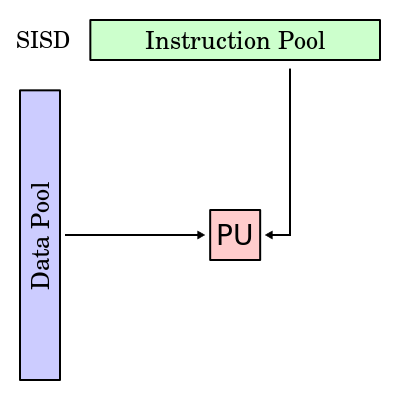
\includegraphics[width=0.25\textwidth,keepaspectratio=true]{images/SISD.png}}
  \subfloat[SIMD]{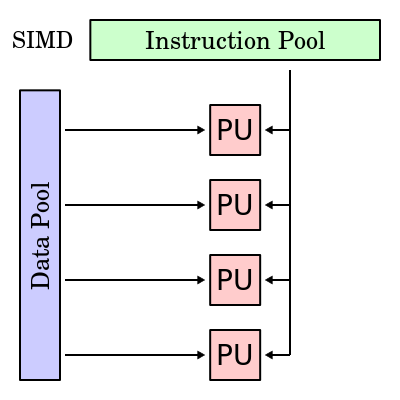
\includegraphics[width=0.25\textwidth,keepaspectratio=true]{images/SIMD.png}}
  \\
  \subfloat[MISD]{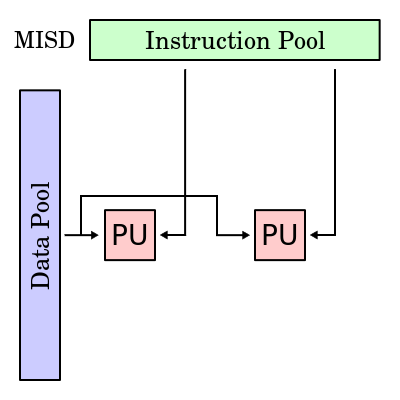
\includegraphics[width=0.25\textwidth,keepaspectratio=true]{images/MISD.png}}
  \subfloat[MIMD]{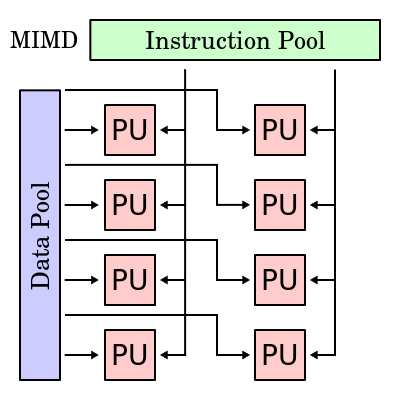
\includegraphics[width=0.25\textwidth,keepaspectratio=true]{images/MIMD.png}}
  \caption{Flynn's Taxonomy of Parallel Computing Systems}
  \label{fig:FlynnsTaxonomy}
\end{figure}

\begin{figure}[h!]
  \begin{minipage}{\textwidth}
\begin{tabularx}{\textwidth}{|c|p{7.5cm}|X|}
  \hline
  Class&Description&Example\\ \hline
  SISD&Single Instruction, Single Data Stream&Traditional Serial Processing\nomenclature{SISD}{Single Instruction, Single Data Stream}\\
  SIMD&Single Instruction, Multiple Data Stream&GPGPU\footnote{Not really any more, but we're getting to that}/Many-core\nomenclature{SIMD}{Single Instruction, Multiple Data Stream}\\
  MISD&Multiple Instruction, Single Data Stream&(Rare\footnote{This architecture is generally only applied where redundancy is critical, and the 'Multiple Instructions' operate on the signal data stream and must agree. One prominent example is the Space Shuttle Flight Control systems})\nomenclature{MISD}{Multiple Instruction, Single Data Stream}\\
  MIMD&Multiple Instruction, Multiple Data Stream&Cluster/Grid systems (e.g. LHCGrid)\nomenclature{MIMD}{Multiple Instruction, Multiple Data Stream}\\
  \hline
\end{tabularx}\caption{Flynn's Taxonomy of Parallel Computation}\label{tab:flynn}
\end{minipage}
\end{figure}

Intuitively, this breakdown is a matrix of data and instruction parallelism. Taking SISD and SIMD separately (as they are the most familiar and relevant), SISD performs a single operation on a single piece of data. It can only process that one piece of data at a time, and can only execute one instruction at a time\footnote{Don't worry dear readers, pipe-lining is coming...}. SIMD on the other hand takes that one execution instruction, and can operate on many pieces of data, producing many results in parallel. This behaviour is augmented in MIMD, where data and instructions are processed in parallel; this could be within a single device (Such as the Cell Broadband Engine) or distributed across the globe.

Flynn created a very clear and simple map of parallelism. Unfortunately the real world got in the way and complicated things. Two major 'complications' will be addressed that have muddied the taxonomic water; SISD Instruction Pipe-lining, and Single Program Multiple Data (SPMD\nomenclature{SPMD}{Single Program Multiple Data Stream}) execution.

\subsubsection{Pipe-lining}
Computer processors are not monolithic boxes that have data pumped into them and the results instantly come out; within even a basic microprocessor, there are a variety of hardware sections that work in sequence, making data and instructions flow through the device to produce the correct result. This sequence is termed the 'pipeline'.

A Generic pipeline consists of four steps;
\begin{enumerate}
  \item Fetch
  \item Decode
  \item Execute
  \item Write-back
\end{enumerate}

Simply put, Fetch grabs the next instruction to be executed from local memory, Decode processes that instruction, prepares the processor's Arithmetic Logic Unit (ALU) for execution, as well as establishing appropriate data I/O memory channels. During Execute, the calculation is performed, and during Write-back, the result of the calculation is stored back in memory. For the sake of simplicity it can be assumed that each of these stages takes one clock cycle.
These tasks are performed by different areas of the chip. This opens up the possibility of having multiple instruction pipelines 'running' at once; 

\begin{figure}[h!]
  \centering
  \subfloat{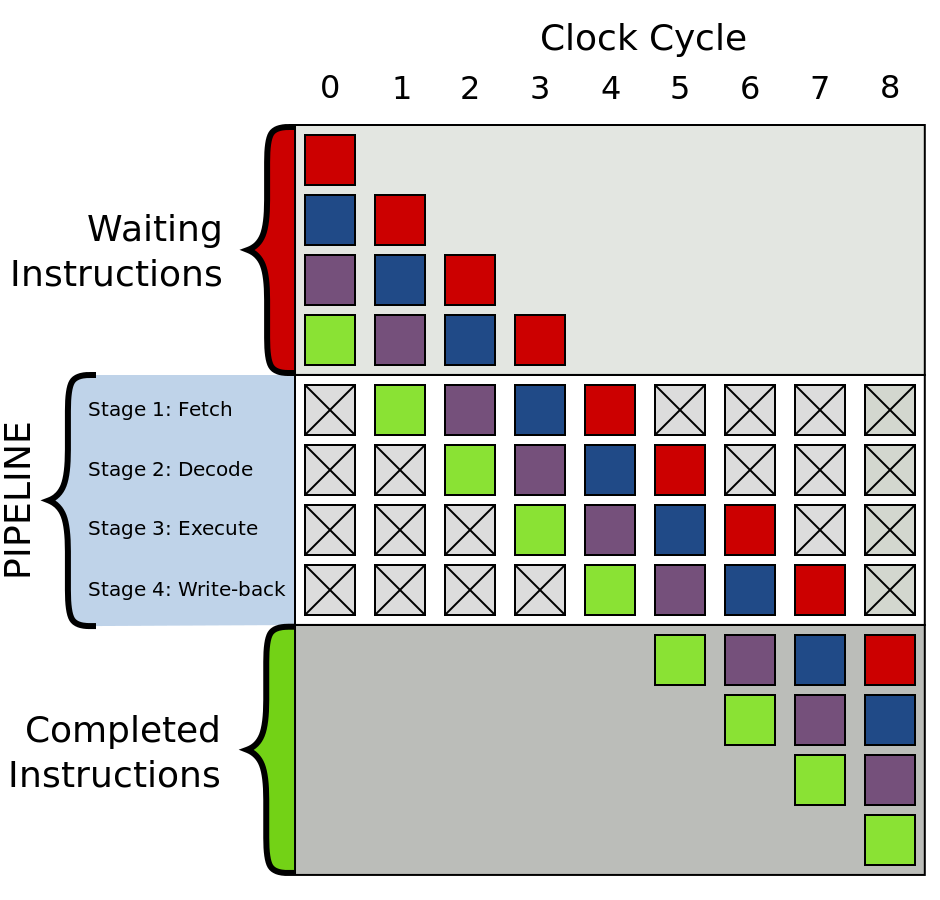
\includegraphics[width=0.4\textwidth,keepaspectratio=true]{images/Pipeline.png}}
  \caption{Example of a 4 Stage Pipeline system}
  \label{fig:Pipeline}
\end{figure}

Looking back to Flynn's Taxonomy, it appears at first glance that what was previously a solid SISD processor could be considered MIMD; the data fetched can be different for each pipelined instruction, and those instructions do not have to be the same either. Whether this counts as true parallelism or not is not as important as its performance improvement; where previously one instruction took four clock cycles to execute, with this simple four stage pipeline, four instructions can be processed in 8 clock cycles.\footnote{Complications to this system arise if the instructions processed are conditional, but as pipe-lining is not the focus of this project, refer to \cite{Yeh91} for more information}

\subsubsection{Single Program Multiple Data}
SISD implementations, at least as developed when Flynn stated his Taxonomy, meant that each machine-level instruction was executed in parallel in lock-step. This meant that data-dependent conditional execution simply wasn't possible without suspending the operation of PUs for which that condition was not satisfied.
SPMD is a subset of MIMD whereby each PU can continue on at its own execution pace, regardless of the state of other PUs. This is exemplified in the Message Passing Interface (MPI\nomenclature{MPI}{Message Passing Interface}) model, where by a (usually) identical program is executed by all PUs, and to control collective program flow and distribution of data, messages are send and received asynchronously between PUs. These PUs could be processor cores within a single machine, or indeed on the same, multi-threading, core, or they could be on machines on opposite sides of the globe.
To add more confusion, in the strictest sense, GPU execution (at least under CUDA) is another different form of parallelism; Single Instruction Multiple Thread (SIMT\nomenclature{SIMT}{Single Instruction Multiple Thread Stream}), which can be though of as a blend of SPMD and SIMD, whereby execution is done is collections of threads simultaneously, and within these collections, instructions are carried out in lock-step as in SIMD, but these collections can be swapped in and out from execution for a variety of reasons, and reorganised based on run-time decisions and resource requirements. The subtleties of this will be discussed in Section ~\ref{fig:CUDAExecArch}.

\subsection{Principles of Parallel Programming}
The concept of splitting a problem set up for separate execution is intuitively simple but in practise very difficult, and has been the major stumbling block in terms of widespread adoption of the parallel programming paradigm. But the potential performance gains afforded from even rudimentary parallelism can be astounding when applied to real world problems.

Examples of problems that are inherently parallel can be found all over the natural and mathematical world; Climate systems can be modelled as atmospheric cells that respond to changes in their surroundings, as can Computational Fluid Dynamics (CFD) and particle physics; Image processing, such as real time video compression can enjoy massive gains as sectors of a video stream can be isolated and processed independently; Linear Algebra, and anywhere where linear algebra is applied\footnote{It's everywhere} is extremely parallelisable in higher-order matrices.

\subsubsection{Gustafson and Amdahl's laws}
Performance improvements from parallelism are not perfect however, as any problem will still retain some operations that are inherently serial.

This limitation has been codified by Gene Amdahl in the law that takes his name\cite{Amd67}, which states that this serial portion of the problem, however small, will limit the overall speed-up provided from parallising the problem. This is stated mathematically in equation ~\eqref{fig:AmdahlsLaw}, where \(\alpha\)\nomenclature{\(\alpha\)}{Fraction of an application that cannot be parallelised} represents the fraction of the program that cannot be parallelised, and graphically in Figure ~\ref{fig:AmdahlFigure}. It is colloquially phrased as:

\begin{quotation}
When a task cannot be partitioned because of sequential constraints, the application of more effort has no effect on the schedule; The bearing of a child takes nine months, no matter how many woman are assigned
\end{quotation}

\begin{equation}
\label{fig:AmdahlsLaw}
S=\frac{1}{\alpha}
\end{equation}

\begin{figure}[h!]
  \centering
  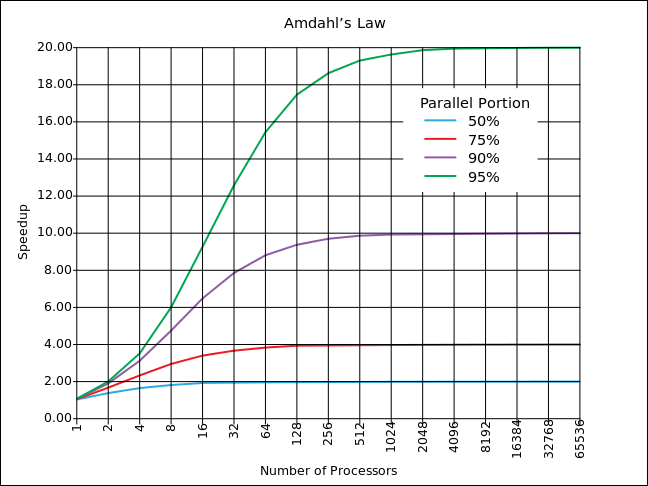
\includegraphics[width=0.75\textwidth,keepaspectratio=true]{images/AmdahlsLaw.png}
  \caption{Graph demonstrating the maximum speed-up attained with a variety of parallelisable program ratios under Amdahl's Law}
  \label{fig:AmdahlFigure}
\end{figure}


Amdahl's Law assumes that the execution time of the non-parallelisable section of the problem is independent of the number of processors available to the system, and that the problem size is fixed. Gustafson's Law\cite{JLG88} at least partially contradicts Amdahl's Law, by stating that for problems with large datasets, parallelisation is still a worthwhile pursuit, regardless of the sequential portion; effectively implying that while parallelism can't make such problems 'faster', the size of their tractable problem sets can be increased if the serial section does not 'slow down' with the problem set size increasing. This is stated mathematically in ~\eqref{fig:GustafsonsLaw} , where \(P\) is the number of processing units available, and graphically in Figure ~\ref{fig:GustafsonFigure}.

\begin{equation}\label{fig:GustafsonsLaw}
S(P)=P-\alpha(P-1)
\end{equation}

\begin{figure}[h!]
  \centering
  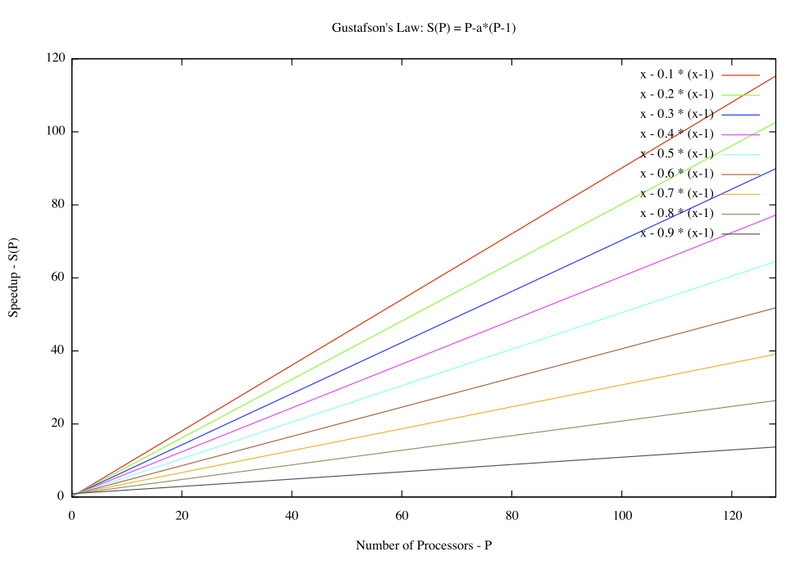
\includegraphics[width=0.\textwidth,keepaspectratio=true]{images/GustafsonsLaw.png}
  \caption{Graph demonstrating the maximum speed-up attained with a variety of parallelisable program ratios under Gustafson's Law}
  \label{fig:GustafsonFigure}
\end{figure}

The both of these Laws are purely theoretical, and do not include aspects of computation such as communication time between PUs, Memory constraints leading to cache contention\footnote{Whereby working data is partitioned across PUs, and in order to maintain the integrity of these caches with respect to the global data state, additional processing is required} or simple processing over-heads involved in running multiple PUs. As such, these Laws can only act as an upper limit to the possible performance of Parallel systems.

\subsection{General Purpose computing on Graphics Processing Units}
\label{sec:GPGPU}
Graphics Processing Units were specialised co-processors designed for real-time image processing and generation, with a focus on the fast growing video game industry. The general architecture of GPU's was designed to perform massive numbers of floating point calculations on each video frame, simulating lighting, texturing, and collision detection events for display devices. This led to quite unique design practices in terms of memory management and execution structures. To put this in perspective, main memory access bandwidth from a High End CPU currently stands at approximately 50GB/s\cite{Var11}, a third of the bandwidth of a similar-generation GPU\cite{NC10}. The idea being that graphics textures are being read many many times over by the collection of PUs, and so needs to be fast.

Around the late 1990's, as this type of hardware became very common on even private desktop machines, the scientific computing community began to use these devices for accelerating highly complex simulations and problems. Up until 2007, in order to accomplish this, the scientific computing problem would have to be 'rephrased' into a graphical problem, utilising a graphics API\footnote{Application Programming Interface\nomenclature{API}{Application Programming Interface}: DirectX and OpenGL allowed game developers to have a hardware-agnostic interface to leverage GPUs and other hardware} such as DirectX or OpenGL. This meant that problems such as matrix multiplication had to be rephrased as overlays of transparent textures, as a contrived example. Taking larger more abstract computational problems and decomposing them into graphical operations was far from simple, and was a major block for many institutions with a desire to use these highly parallel devices.

In 2007, NVIDIA released a new reference architecture for its high-end graphics cards, specifically aimed at the scientific and application-acceleration communities; the Compute Unified Device Architecture (CUDA)\cite{NC07}. CUDA was not just a new C/C++/FORTRAN API, exposing low-level execution and memory control to scientific computing, but was a complete re-write of all intermediate software layers, and included the addition of specific interface hardware, along side the standard graphics interface, dedicated for CUDA computing\cite{DBK10}, see Figure ~\ref{fig:CUDAArch}. In 2007, one GPU chip-set supported CUDA; the G80. In 2008, The Tokyo Institute of Technology's TSUBAME supercomputer became the first GPU accelerated machine in the Top500 World Supercomputer rankings\footnote{TSUBAME made it to 29th in the world rankings, with the addition of 170 Tesla S1070 systems\cite{Hum08}}. By 2011, over 20 different chipsets encompassing over 40 individual manufacturer cards and hundreds of after-market cards, constituting over 100 million CUDA-enabled cards\cite{iVE10} sold across the globe.

In 2008, Apple Inc, in collaboration with NVidia, Intel, IBM and AMD released a C/C++ based framework for mixed CPU/GPU/Manycore/FPGA heterogeneous computing called OpenCL (Open Computing Language). OpenCL contains much more programming abstraction away from the hardware compared to pure-CUDA, and as such cannot be as highly optimised. Even still, NVidia rolled out agnostic device interfaces to OpenCL. The current CUDA architecture is shown in Figure ~\ref{fig:CUDAArch}

\begin{figure}[h!]
\centering
  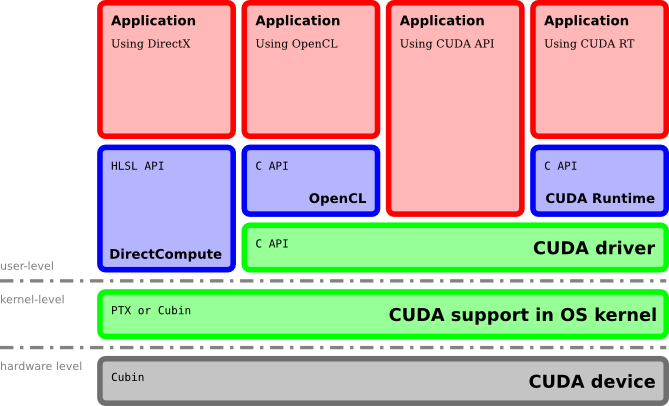
\includegraphics[width=0.75\textwidth,keepaspectratio=true]{images/cuda_architecture.png}
  \caption{Diagram showing levels of abstraction between Hardware and various APIs}
  \label{fig:CUDAArch}
\end{figure}

\subsection{CUDA Execution architecture}\label{fig:CUDAExecArch}
A CUDA execution consists of both host (CPU) and device (GPU) phases. The device phases, called kernels, are written in C/C++\footnote{As we'll see, wrappers for other languages exist, but there is always an intermediate C/C++ stage}. Since these kernels reside only on the device, access to main host memory is impossible, and data sets to be worked on, as well as areas of memory to store results, must be set-up by the host on the device before invocation. The amount of parallelism used by the kernel is decided per-kernel invocation, but the kernels themselves must be written with this level of parallelism in mind; there are no magic tricks in CUDA. To understand this, the low level architecture of the GPU must be investigated. 

\begin{figure}[h!]
  \centering
  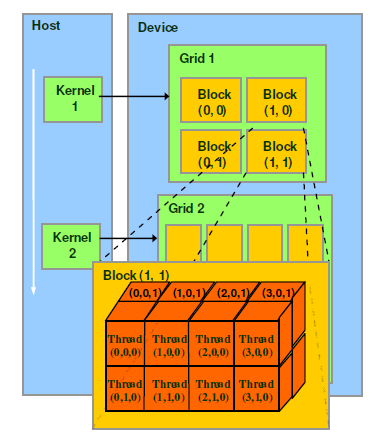
\includegraphics[width=0.45\textwidth,keepaspectratio=true]{images/CUDA_host_dev_threads.png}
  \caption{Diagram showing levels of execution between host and CUDA device operations}
  \label{fig:CUDAHostDevExec}
\end{figure}

Starting from the top down, a host machine can have multiple GPU devices, which can all be individually addressed for asynchronous execution in parallel. Below this level, and as shown in Figure ~\ref{fig:CUDAHostDevExec}, there are logical 'Grids', which contain logical 'Blocks' of threads. These Grids and Blocks are the fundamental form of execution parallelism. As shown in Figure ~\ref{fig:CUDAHostDevExec}, Grids can be thought of as two dimensional arrays of Blocks, and Blocks are thought of as three dimensional arrays of Threads. It is these threads that actually execute any particular workload.

\begin{figure}[!h]
  \centering
    \begin{lstlisting}[numbers=left, language=C, numberstyle=\tiny, numbersep=8pt]
    //Setup dimensions of grids and blocks
    dim3 blocksPerGrid(65535,1,1);
    dim3 threadsPerBlock(64,8,1);

    //Invoke Kernel
    kernelfunction<<<blocksPerGrid,threadsPerBlock>>>(*functionarguments);
    \end{lstlisting}
  \caption{Example CUDA host code segment, showing kernel invocation}
  \label{fig:KernelInvocation}
\end{figure}

As stated, the level of parallelism is defined at the kernel invocation stage and (until very recently\footnote{The latest Fermi devices support multiple parallel kernel invocations, under which SMs are assigned different kernels based on a proprietary load-balancing algorithm}) only one kernel can run on a single device at a time. Following the SIMD model, parallelism is attained by per-thread self-indexing. In the case of CUDA, each thread could generate a unique 1D execution index using a combination of runtime variables that are pro grammatically exposed through the CUDA Driver API, as shown in Figure ~\ref{fig:GridBlockThread1D}. In this particular example, it assumed that both Grid and Block dimensions are 1D. This is useful in this case for scalar multiplication of linear arrays, and could process input data containing \(2^{16}\times 2^{10} = 2^{27}\), or over 67 million values\footnote{For the latest generation of Tesla GPUs}. CUDA introduces several additional keywords to the C language, in this case "\_\_global\_\_", which indicates that the function is executed on the device, but can be called from the host. A summary of these function declaration keywords is shown in Table ~\ref{tab:CUDAFuncDecTable}

\begin{figure}[!h]
  \centering
    \begin{lstlisting}[numbers=left, language=C, numberstyle=\tiny, numbersep=8pt]
    __global__ void multArray(float *array, float multiplier){
      int 1Dindex = blockIdx.x*blockDim.x+threadIdx.x;
      array[1Dindex]=array[1Dindex]*multiplier;
    }
    \end{lstlisting}
  \caption{Example CUDA kernel, showing 1D index identification}
  \label{fig:GridBlockThread1D}
\end{figure}


\begin{table}[!ht]
\begin{tabularx}{\textwidth}{|X|c|c|}
Function Declaration&Executed by&Callable From\\\hline
\_\_device\_\_ void someKernel&device&device\\
\_\_global\_\_ void someKernel&device&host\\
\_\_host\_\_ void someKernel&host&host\\
\end{tabularx}
\caption{Table of CUDA Function Declaration Keywords and their use}\label{tab:CUDAFuncDecTable}
\end{table}

For more parallelism, and more context relevance, consider scalar multiplication of large matrices. The previously stated indexing scheme could be used sequentially, i.e taking each row of the matrix in turn and farming the computation of that row to the GPU, but as stated, CUDA allows (actually encourages) multi-dimensional indexing, so each thread execution could be tasked with modifying multiplying one matrix element by 2D addressing, as shown in Figure ~\ref{fig:GridBlockThread2D}. This form of parallelism theoretically allows for up to \(2^{16}*2^{16}*2^{10}*2^{10}=2^{52}\) or about 4.5 quadrillion threads, (i.e operating on a square matrix of side \(2^{27}\))\footnote{Due to Memory and Hardware considerations, this is a ridiculously contrived metric}.

\begin{figure}[!h]
  \centering
    \begin{lstlisting}[numbers=left, language=C, numberstyle=\tiny, numbersep=8pt]
    __global__ void multMatrix(float *matrix, float multiplier){
      int x_index = blockIdx.x*blockDim.x+threadIdx.x*;
      int y_index = blockIdx.y*blockDim.y+threadIdx.y*;
      matrix[x_index][y_index]=matrix[x_index][y_index]*multiplier;
    }
    \end{lstlisting}
  \caption{Example CUDA kernel, showing 2D index identification}
  \label{fig:GridBlockThread2D}
\end{figure}

Moving into the practical realm, once a kernel is launched, the CUDA runtime system generates the corresponding logical grid of threads. These threads are assigned to execution resources such as shared memories and thread registers\footnote{These will be covered in detail in Section ~\ref{fig:CUDAMemArch}} on a block-by-block basis\footnote{For the sake of simplicity, the following section discusses the hardware capabilities of the latest generation of Fermi cards, specifically the Tesla C2050 Workstation card}. These resources are organised into streaming multiprocessors (SMs), the number of which vary depending on the particular hardware, but usually around 15 are active. These SMs can each be assigned up to 32 thread-blocks, each of which is executed on a separate Streaming Processor (SP) core. These cores can handle up to 48 threads in parallel. In the case of the Tesla C2050, this means that over 20,000 threads can be 'simultaneously' executed.

Note that this does not limit the grid and block dimensions; groups of threads, termed warps, are swapped in and out of the SM's regularly, making execution tolerant of long-latency operations such as global memory access. This warping of threads is also an important concept for thread-divergence; when runtime-dependant conditional statements in kernel execution have different branching behaviours in threads that are in the same 'warp', the warp is actually executed twice; once for the major condition, and once for the minor condition. Between these two executions, the results obtained from the 'minor' path are discarded and during the minor execution, the results from the major path are also discarded. It is for this reason that conditional behaviour should be avoided in a GPU environment (Figure ~\ref{fig:thread-divergence} demonstrates this. Adapted from \cite{KF08}). 

\begin{figure}[h!]
  \centering
  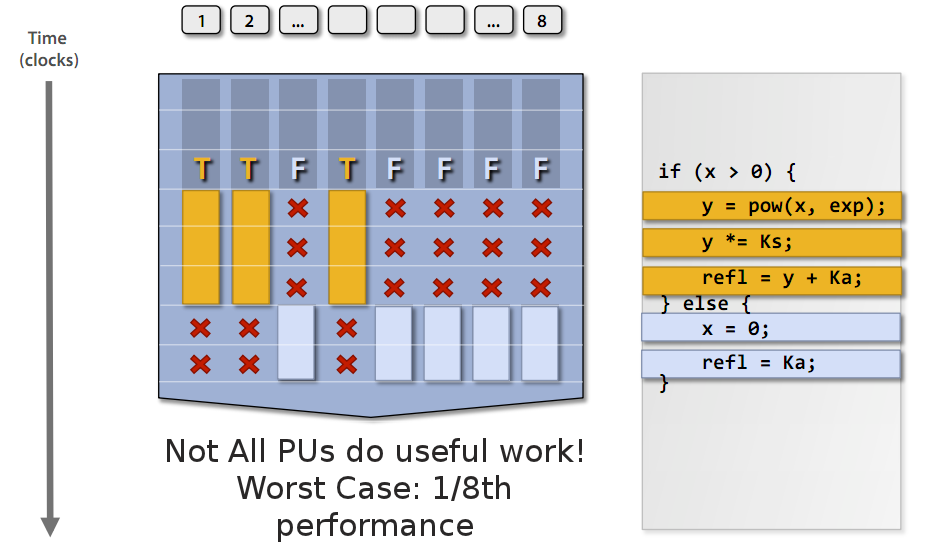
\includegraphics[width=0.75\textwidth,keepaspectratio=true]{images/thread_divergence.png}
  \caption{Diagram showing thread divergence operation under CUDA, adapted from SIGGRAPH 2008 proceedings}
  \label{fig:thread-divergence}
\end{figure}

As mentioned, resource allocation is partially decided upon the memory requirements of a particular kernel. These and other memory related concepts are covered in the following section.

\subsection{CUDA Memory architecture}
Utilising the levels of parallelism demonstrated previously, one would expect massive performance improvements to be a given. This is not the case, and 'lazily parallelised' applications generally achieve only a small fraction of the potential speed of the underlying hardware, and most of the time, the limiting factor is memory latency. To understand why this is the case, it is important to investigate the CUDA memory architecture.

CUDA devices have three major levels of memory; Thread local, Block Shared, or Grid Global. This architecture is displayed diagrammatically in Figure ~\ref{fig:CUDAMemArch}, and summarised in Table ~\ref{tab:CUDAMemTable}.

\begin{figure}[h!]
  \centering
  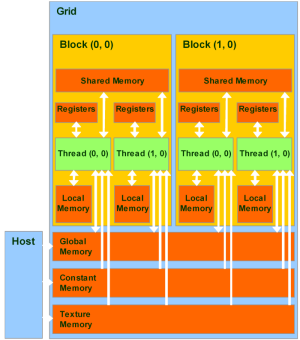
\includegraphics[width=0.5\textwidth,keepaspectratio=true]{images/cuda_mem_arch.png}
  \caption{Diagram showing CUDA memory access architecture}
  \label{fig:CUDAMemArch}
\end{figure}

\begin{table}[!ht]
\begin{tabularx}{\textwidth}{|c|c|c|c|X|c|}\hline
Memory&Scope&Lifetime&R/W&Usage&Speed\\\hline
Register&Thread&Kernel&R/W&Automatic variables other than arrays&Very Fast\\
Local&Thread&Kernel&R/W&Automatic Array Variables&Very Fast\\\hline
Shared&Block&Kernel&R/W&\_\_shared\_\_&Fast\\\hline
Global&Grid&Application&R/W&Default&Very Slow\\
Constant&Grid&Application&R&\_\_constant\_\_&Slow\\\hline
\end{tabularx}
\caption{Table of CUDA Memories and some characteristics}
\label{tab:CUDAMemTable}
\end{table}

In order to get data to and from the device, Global, Constant and Texture memory is read-write accessible from the host; any other memory allocation is done on a per-thread basis.

Texture memory is a particular area of constantly declared memory that is logically represented as a 2D array, and is augmented with a distributed cache of 2D localised values from last access and as such is significantly faster than Global memory. This behaviour is particularly useful for applications such as linear algebra and CFD.

Due to their scientific ubiquity, parallelisation of linear algebra systems is a heavily researched field, leading to highly customised libraries available, such as BLAS (Basic Linear Algebra Subprograms) and MKL (Math Kernel Library). cuBLAS is a CUDA library specifically optimised for most Level 1, 2, and 3 BLAS functions running on GPU, and this library and others like is is heavily used within the research community\cite{MF08}.

This competitive optimisation in all linear algebra systems means that defined linear algebra functions are a natural benchmark for cross-comparison between parallel CPU and GPU implementations; each candidate library doing the best they can do with the hardware. And frankly, GPU wipes the floor with CPU, as in Figure ~\ref{fig:BLASComp}.

\begin{figure}[h!]
\centering
    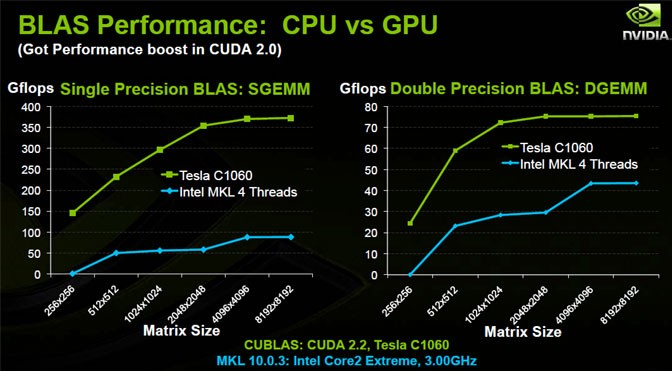
\includegraphics[width=0.75\textwidth,keepaspectratio=true]{images/NVDA_BLAS_C1060_vs_CPU_675.png}
  \caption{Image Courtesy of NVidia Corp. Showing CPU/GPU comparison of highly optimised BLAS libraries}
  \label{fig:BLASComp}
\end{figure}

In \cite{DBK10}, a variety of matrix multiplication kernels designed for matrices of many thousands of elements are shown with a variety of optimisations. A Naive implementation is shown, as in Figure ~\ref{fig:MatMulNaive} that performs at (only) 17.2 GFLOPS\footnote{Giga-Floating Point Operations per Second}. With a few modifications, a similar kernel (Figure ~\ref{fig:MatMulShare}) can perform at 47.5 GFLOPS; nearly 280\% faster. The major modification is the use of what is called 'shared' memory, i.e memory that is common to a thread-block.

In Figure ~\ref{fig:MatMulNaive}; matrix pointers \(A, B, C\) point to the two input and one output matrix respectively, where global memory has been allocated and moved onto the device by the host application, and the kernel is invoked with the width of the matrix to stay in memory bounds. Each block of threads will calculate a section of the output matrix, as shown in Figure ~\ref{fig:MatMulNaiveDiag}.

\begin{figure}[!h]
  \centering
    \begin{lstlisting}[numbers=left, language=C, numberstyle=\tiny, numbersep=8pt]
      __global__ void matmulNaive(float *A, float *B, float *C, int WIDTH){
        Tx = threadIdx.x; Ty = threadIdx.y;
        Bx = blockIdx.x; By = blockIdx.y;

        X = Bx * blockDim.x + Tx;
        Y = By * blockDim.y + Ty;

        idxA = Y * WIDTH;   
        idxB = X;
        idxC = Y * WIDTH + X;

        Csub = 0.0;

        for (i=0; I < WIDTH; i++) {
          Csub += A[idxA] * B[idxB];
          idxA += 1;
          idxB += WIDTH;
        }

        C[idxC] = Csub;
      }
    \end{lstlisting}
  \caption{Example CUDA kernel, showing Naive parallel matrix multiplication with Global memory access}
  \label{fig:MatMulNaive}
\end{figure}

\begin{figure}[h!]
\centering
  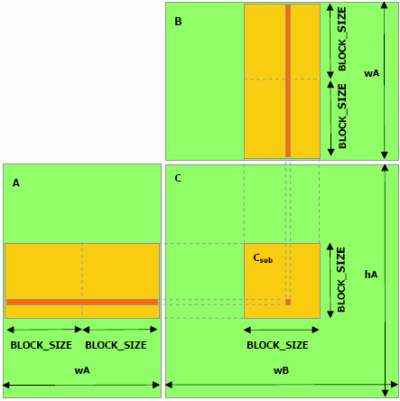
\includegraphics[width=0.45\textwidth,keepaspectratio=true]{images/naive_matrix.png}
  \caption{Naive matrix calculation with memory access by a single block highlighted}
  \label{fig:MatMulNaiveDiag}
\end{figure}

In this example, every access to A, B, or C (lines 15 and 20) is from/to Global memory. This access is orders of magnitude slower than the access to thread-local variables such as the A and B indexes. One improvement that can be made initially is to use block-shared memory. This is demonstrated in Figure ~\ref{fig:MatMulShare}. In this case, each thread retrieves one element from each input array, and stores it in block-shared memory, i.e the threads collaboratively copy the data required for whole-block execution. Note the \_\_syncthreads() in lines 19 and 22; this CUDA call instructs each thread in the block to wait for all other threads in the block to come to the same execution point before continuing. In this case this is to ensure that all of the relevant elements have been copied by all of the block-warps before trying to do any actual calculations. The operation is similar to previous, as shown in Figure ~\ref{fig:MatMulNaiveDiag}, except that the outer while loop makes each thread 'step' across the input matrices. This has the effect of greatly reducing the number of Global memory accesses, and has the added benefit of increasing what is called coalesced memory access.

\begin{figure}[!h]
  \centering
    \begin{lstlisting}[numbers=left, language=C, numberstyle=\tiny, numbersep=8pt]

        __shared__ float As[blockDim.x][blockDim.y];
        __shared__ float Bs[blockDim.y][blockDim.x];
        Csub = 0.0;
        Tx = threadIdx.x; Ty = threadIdx.y;
        Bx = blockIdx.x; By = blockIdx.y;

        X = Bx * blockDim.x + Tx;
        Y = By * blockDim.y + Ty;

        idxA = Y * WIDTH;   
        idxB = X;
        idxC = Y * WIDTH + X;

        while (idxA<WIDTH) {  // iterate across tiles
          As[Ty][Tx] = A[idxA];
          Bs[Ty][Tx] = B[idxB];
          idxA += blockDim.x;  idxB += blockDim.y * WIDTH;
          __syncthreads();
          for (i=0; i < 16; i++) {
            Csub += As[Ty][i] * Bs[i][Tx];
            __syncthreads();
          }
        }
        C[idxC] = Csub
    \end{lstlisting}
  \caption{Example CUDA kernel, showing Naive parallel matrix multiplication with Shared memory access}
  \label{fig:MatMulShare}
\end{figure}

Coalesced memory accesses are simply batching of memory reads and writes, where all (or most) threads in a warp access a linearly contiguous data space, i.e the \(k^{th}\) thread in a given warp accesses the \(k^{th}\) element of an array. This way, the 'block' SP can perform these reads or writes as one instruction, instead of each individual thread accessing individually. In this case, matrix A accesses are largely coalesced, as each thread is grabbing its own element within a row of A, but B accesses are uncoalesced. One solution, that will not be investigated here, is performing an transpose on B and then performing the more complex multiplication; this operation would only be useful for fairly large Matrices.

Looking beyond shared memory and memory coalescing schemes schemes, CUDA exposes many memory access interfaces for handling different arrangements of data, and for more detailed information refer to \cite{NC11}.

In summary, the performance of CUDA, and generally any, parallel application is dependant on many factors; from efficient runtime resource allocation; memory types and access techniques; and most importantly, input data dimensions. This is demonstrated when matrix multiplication algorithms are used applied to 'smaller' matrices; Figure ~\ref{fig:CPU_GPU_MATMUL_SMALL} shows that for small matrices, \(N~180\), CPU-bound calculation is significantly more performant than GPU-bound solutions. From this section it is clear why this is so; memory latency, kernel processing overheads, and a minimal workload all work against a parallelised GPU implementation. Where the problem set is large, for instance, warp-swapping is used to continue to efficiently provision resources to queued warps while other warps are waiting on memory retrievals.
This economy of scale is an important design heuristic when developing for GPU and will significantly influence the allocation of work in this project.

\begin{figure}[h!]
\centering
    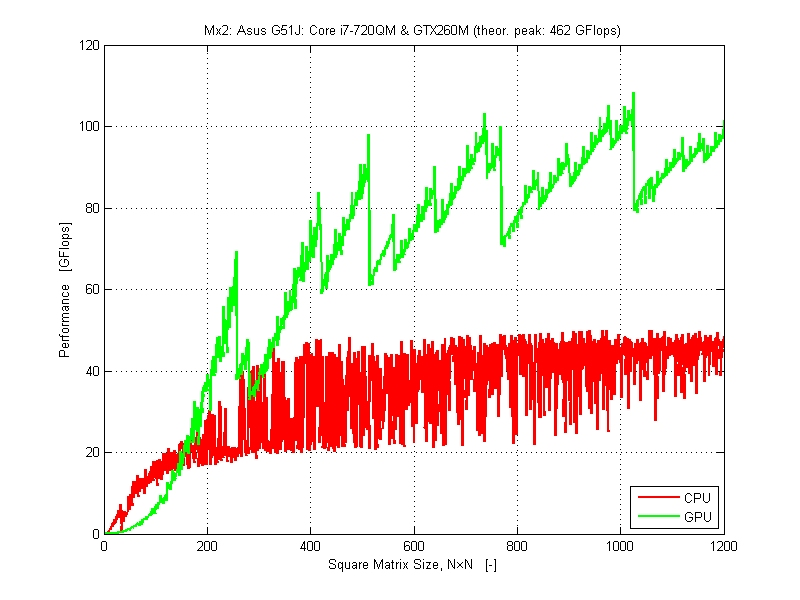
\includegraphics[width=0.75\textwidth,keepaspectratio=true]{images/FlopsMx2_Asus_G51J_02.png}
  \caption{Image Courtesy of AccelerEyes  Showing lower order CPU/GPU comparison of MATLAB Matrix Multiplication using the Jacket framework}
  \label{fig:CPU_GPU_MATMUL_SMALL}
\end{figure}

\section{Opportunities for Parallel Decomposition of DSM Algorithms}
With an understanding of the mathematical challenges presented in the DSM problem, and the current availability of Parallel Computing technologies (specifically those presented by innovations in GPGPU), it is worthwhile to pause and analyse potential decomposition techniques that could be applied to algorithmic acceleration.

In \cite{AM09}, McKinley observes that the majority of computational time accrued in the generation of optimal and near-optimal bit-loading configurations is in the calculation of power spectral densities of candidate bit-loads. This naturally stems from the previously discussed exponential relationship between number of lines, maximum bits-per-tone, and the resultant number of possible bit-combinations. The calculation of PSDs is the solution of \(N\) linear systems, as stated in equation ~\eqref{eq:SysModMat}.

As discussed in Section ~\ref{sec:ParallelComputing}, parallel computation is ideal, especially under the CUDA model, for solving systems of linear equations with high \(N\). The downside is that to utilise parallelism effectively, the number of systems must be quite large (100+, see Figure ~\ref{fig:CPU_GPU_MATMUL_SMALL}). Since in general DSM bundles consist of 50 lines, and range up to 100, there is no rational justification for offloading this work to existing libraries such as cuBLAS, as they will perform significantly worse than equally optimised CPU-bound libraries.

Even so, the small \(N\) also can be an advantage; considering the previously discussed memory architecture of CUDA, it is feasible to create a small, customised, linear system solver that resides in-thread; i.e, each thread solving one small system of equations. 

To restate the DSM problem in general; the process of generating optimal bit-load configurations is a \(N\) dimensional optimisation problem, and as such stands as one of the most difficult problems in computation, which has not completely been 'solved' in either the sequential or parallel realms \cite{JDJZW03}.

This allows a simplified reclassification of the previously discussed DSM algorithms in terms of purely their qualitative searching techniques; OSB exhibits \(N\) dimensional exhaustive search behaviour, ISB exhibits behaviour similar to segmented linear search schemes, and MIPB takes a heuristic increment-and-search approach. 

The range of these behaviours immediately indicates that no 'one-size-fits-all' solution is going to work; each problem will have to be tackled individually.

\subsection{Parallel OSB}
Even though OSB is a computationally explosive searching solution, it would still be worth while to attempt to parallelise it, as it is the 'simplest' of algorithms, and its core can be explained quite simply; For each channel, calculate the PSD's of every possible bit-loading combination, subsequently find the Lagrangian cost for this bit-load scheme on this channel, and thus return the maximally optimal bit-loading combination for the entire bundle on this channel. 

It's clear even from this simple statement that parallelisation will be effective; Each thread can calculate the PSD and subsequent Lagrangian for each bit-combination in parallel, then a reduction can be used to find the maximum Lagrangian and bit-load. This presents a prarallelisation across Channels, Lines, and bit-permutations, and would be relatively simple to leverage multiple devices in this scheme; each device is assigned a channel range or a channel queue, and calculates the local optimisation for the channel, returning its result back to the host.

Intuitively, this should give significant speed-up's for lower numbers of lines (i.e up to 4 or 6), but due to bit-combination-explosion, will remain intractable for higher line counts.

\subsection{Parallel ISB}
ISB segments the search problem of OSB such that instead of searching every possible bit-loading combination for every line, per-user bit-loading is searched on each tone, so that in the lowest level, there are \(O(N^2)\) combinations as opposed to OSB's \(O(2^N)\). After searching a single line, the global bit-load for that line is updated, and the next line is searched. 

From a parallelisation perspective, this global updating of bit-loads is concerning as it creates much more opportunity for memory contingency problems as well as non-optimal SM occupancy where the number of users is relatively small (i.e. below 8), as each line-search will have to wait on the search for the previous line. That said that larger numbers of lines, the problem should be highly scalable by having thread blocks collaboratively searching individual line loads and continuously updating a global record of bit-loads. Indeed there is the possibility of having larger thread blocks that individually search different lambda values in parallel, simplifying bisection search. Another possibility is to invert the ISB looping constructs such that all channels can take one 'step' in parallel.

As such, one would hope for at least channel and bit permutation parallelism, but due to the incremental update nature of ISB, could not exhibit line parallelism. This represents a much smaller parallelisation problem which will be significantly more difficult to shoehorn into a multi-device structure due to data dependency, but one would predict that the combination of reduced computational complexity of ISB, and this style of parallelism, that GPU ISB will be very very fast compared to even GPU OSB.

\subsection{Parallel MIPB}
Due to the sequentially coupled nature of the MIPB algorithm, it is inherently difficult to parallelise effectively. MIPB only needs to update one \(N\) psd vector at each bit-increment, and this could only really be accelerated across \(N\) threads. This factor alone indicates that MIPB may not be directly parallelisable in its simple form, but some future adaptations of MIPB utilising the deterministic nature of 'bit-increment chains' presents an algorithmic possibility of pre-computing the bit-increment paths on each channel and using these weighted increment trees to allocate bit-loads based on power constraints.

In any case, MIPB will be implemented as a CPU bound comparison, with an attempt at a GPU implementation, to assess the comparative merits of for instance GPU ISB/OSB against MIPB.

